\section{Experimental Results}
    In this section, we first present the overall success rate for cracking
    the 120 patterns collected from our participants plus the top 60 most complex patterns
    on a $3\times3$ pattern grid.
    Our results show that our approach can successfully crack over 95\% of the
    patterns using no more than five attempts. We then analyze how the
     success rate is affected by the filming distance, filming angles and
    camera shake. Finally, we demonstrate that direct observations lead to poor
    performance before evaluating our approach on alternative pattern grids.

\begin{figure}[!t]
    \centering
    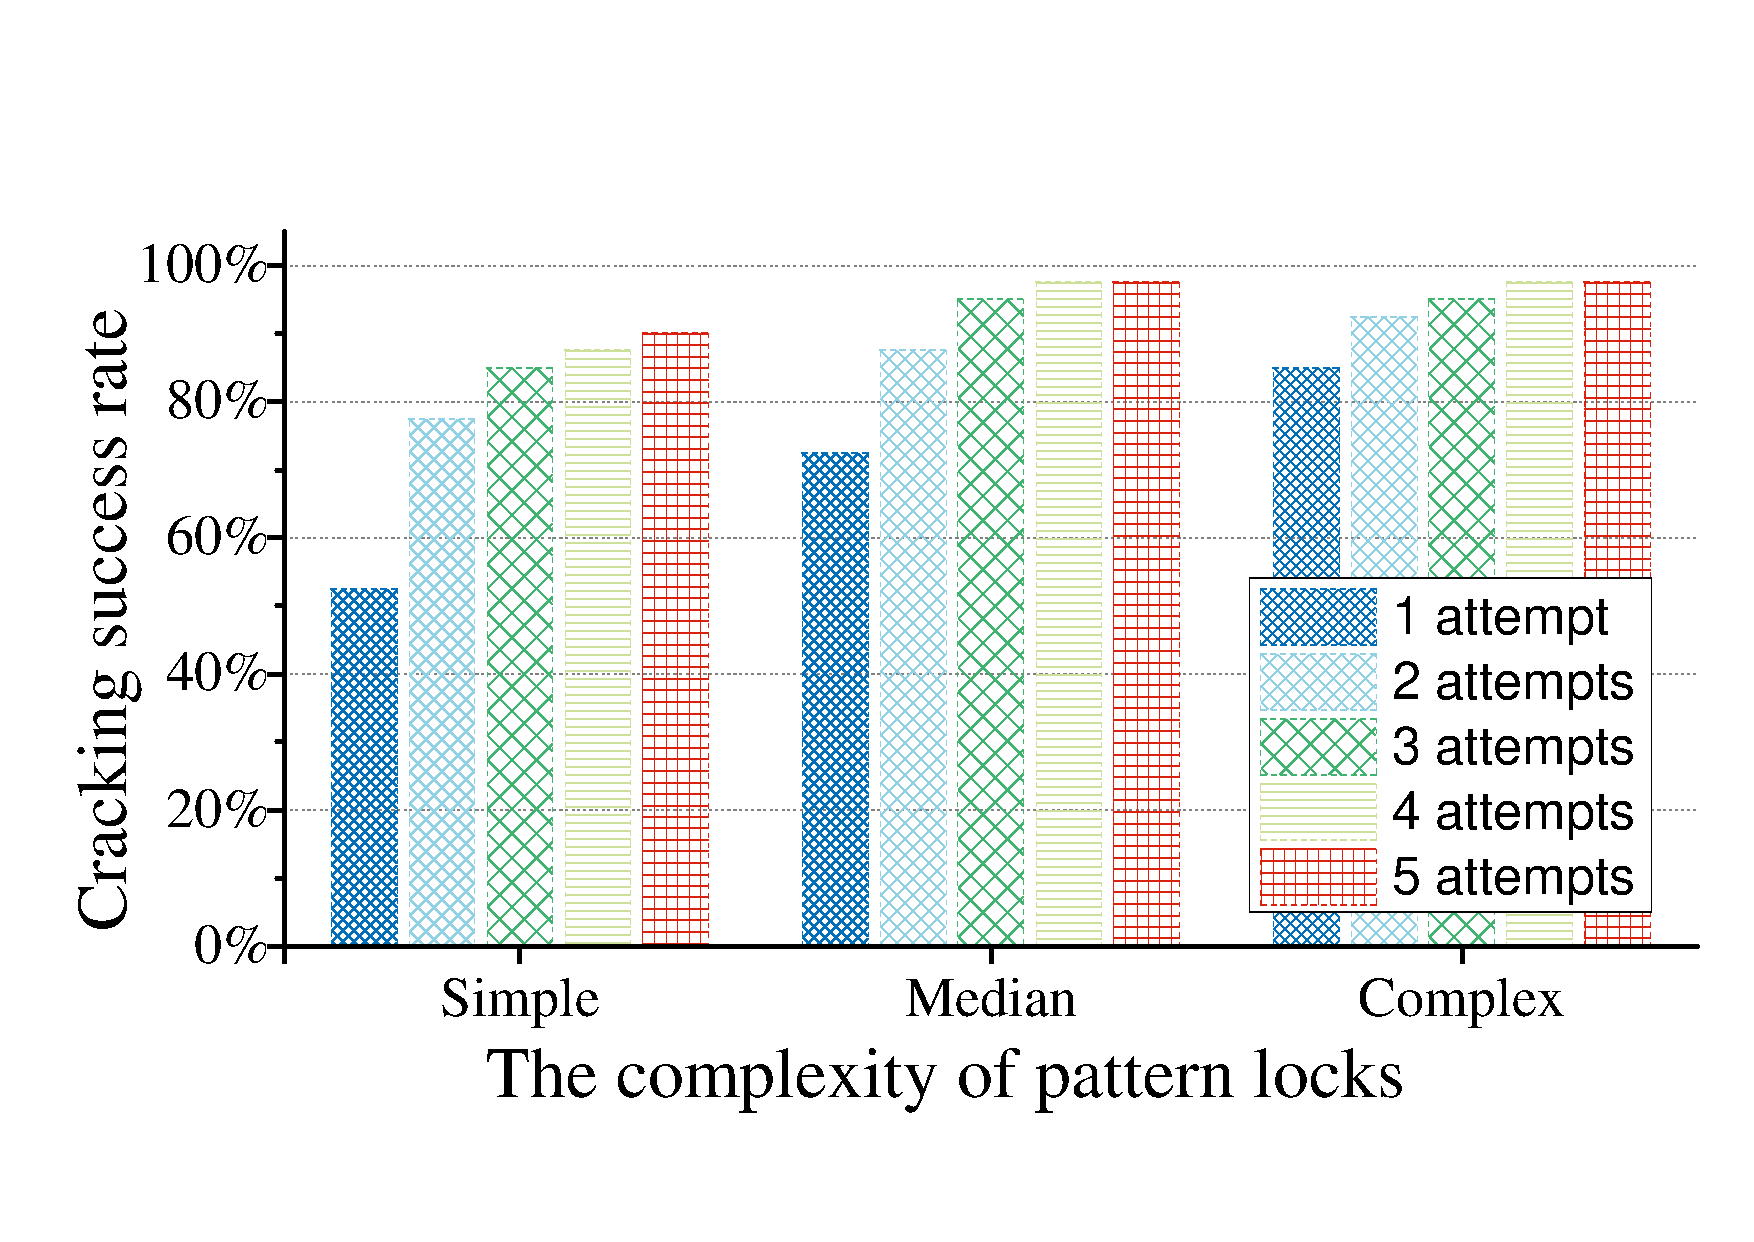
\includegraphics[width=0.35\textwidth]{fig/10.pdf}
    \vspace{-3mm}
    \caption{For each pattern category, the figure shows the success rate using no more than 1, 2, 3, 4 and 5 attempts.}
    \label{fig:fig10}
    \vspace{-2mm}
\end{figure}

    \subsection{Overall Success Rate \label{sec:overall_rate}}

    \noindent \textbf{Result 1:}  \emph{We can successfully crack over 95\% of the patterns in five attempts and complex patterns are less secure compared to simple patterns under our attack.}

        In this experiment, videos were recorded from a distance of 2 meters away
        from the target device. This mimics a scenario where the adversary sits
        at the next table to the user in a public space (e.g. a restaurant).
        The smartphones used for filming in this experiment were hand-held.
        Figure~\ref{fig:fig10}
        shows the success rate for cracking different types of patterns within 1, 2, 3, 4 and 5 attempts.     For all the patterns used in this evaluation,
        our approach does not generate more than  five candidate patterns.
        For complex patterns, we are able to crack all except one in the first attempt.
        For simple and median patterns, the success rate increases with more tries.
        In one attempt, we are able to
        successfully crack 60\% and 87.5\% of the simple and median patterns respectively. With two attempts, the success rate increases to 87.5\%,
        and 95\% for simple and median patterns
        respectively. Using five attempts, we are able to
        crack all simple patterns and all but one median patterns.
       The reason that we failed on one median and one complex patterns is because of some blur motions of the video footage (probably
       caused by the video compressing algorithm), which leads
       to many tracking failures. But we are able to crack the same
       pattern using a video filmed by a different device.
        It is important to note that the Android OS will not lock the device unless seeing
        more than five failed tries~\cite{egelman2014you}. This means, in practice, our approach is able to
        successfully crack most locking patterns.

\begin{figure}[!t]
    \centering
    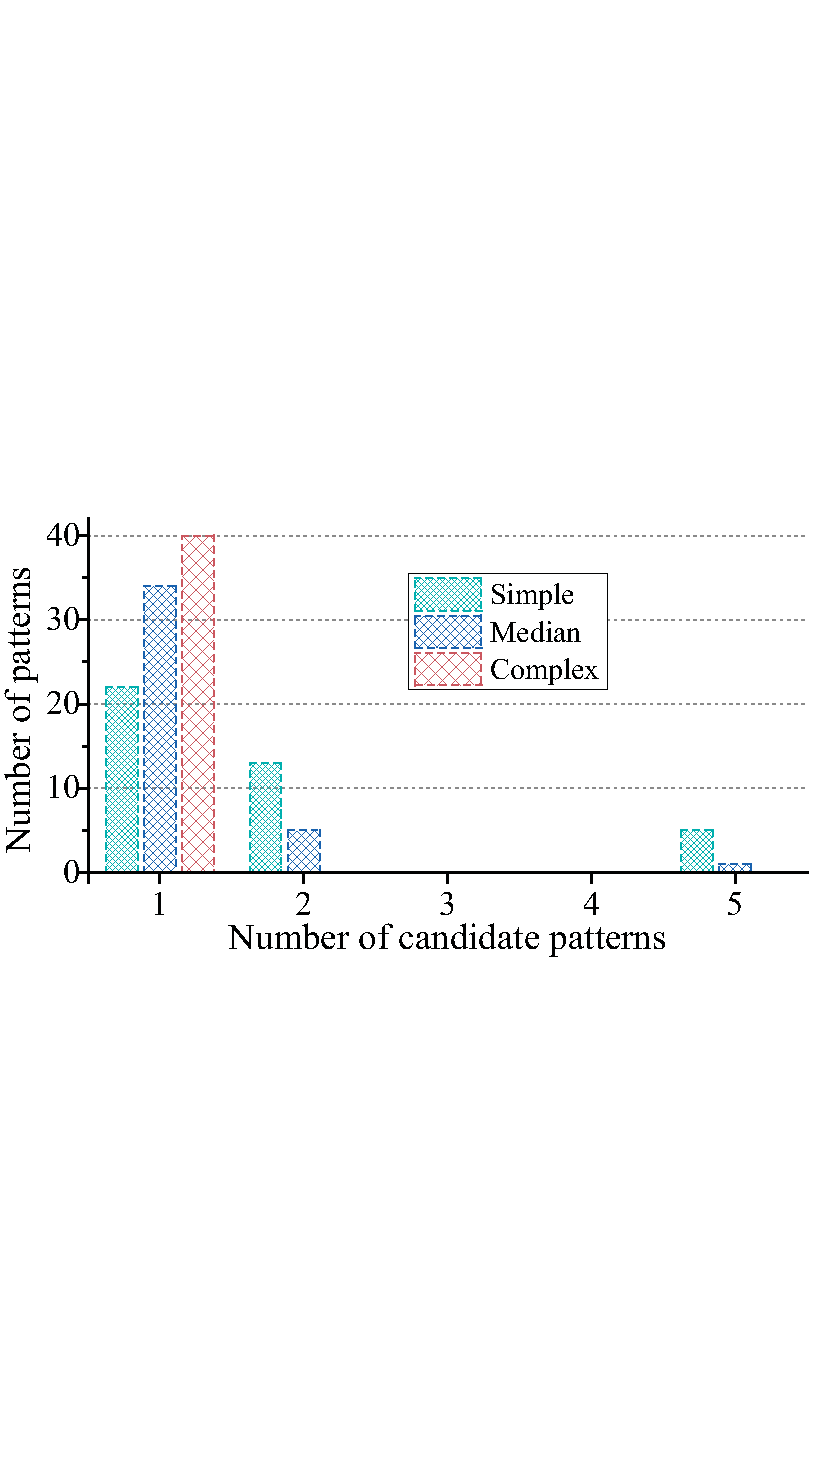
\includegraphics[width=0.35\textwidth]{fig/11.pdf}
    \vspace{-3mm}
    \caption{The distribution of candidate patterns for each category. No more than 5 candidate patterns were generated by our algorithm. }
    \label{fig:fig11}
    \vspace{-2mm}
\end{figure}

        Another interesting observation is that in contrast to many people's
        intuition, complex patterns do not provide stronger protection under our attack because
        most of these patterns can be cracked in one attempt.
        This is because although complex patterns can better protect the user against direct observation techniques like shoulder surfing~\cite{shoulder}, their unique graphical structures
        often allow our system to reject most patterns to produce a single candidate pattern. This is
        confirmed by Figure~\ref{fig:fig11}. It shows that for most median and all complex patterns, our system produces one candidate pattern --
        the correct one for most of our test cases.


       We also evaluated our approach using the top 60 most complex
        patterns (according to Equation~\ref {equ:compscore}) on a $3 \times 3$
        grid.
        To evaluate our approach on a wide range of patterns, we exclude patterns that are simply a rotation to an already chosen pattern.
         Figure~\ref {fig:most complex patterns} illustrates three
        highly complex patterns which have a complexity score between 43.8 and 46.8. The three
        patterns use all the nine dots of the grid and have a larger number of line segments, intersections and overlapping lines when compared to simpler patterns.
        Because of their complex graphical structures, it would be hard to remember
        these patterns using direct observation techniques.
        In this experiment, we can crack all the complex patterns in one attempt. This result reinforces our claim that complex
        patterns are less security under video-based attacks.




    \begin{figure*}[!ht]
            \centering
            \subfigure{
                \begin{minipage}[b]{3.8cm}
                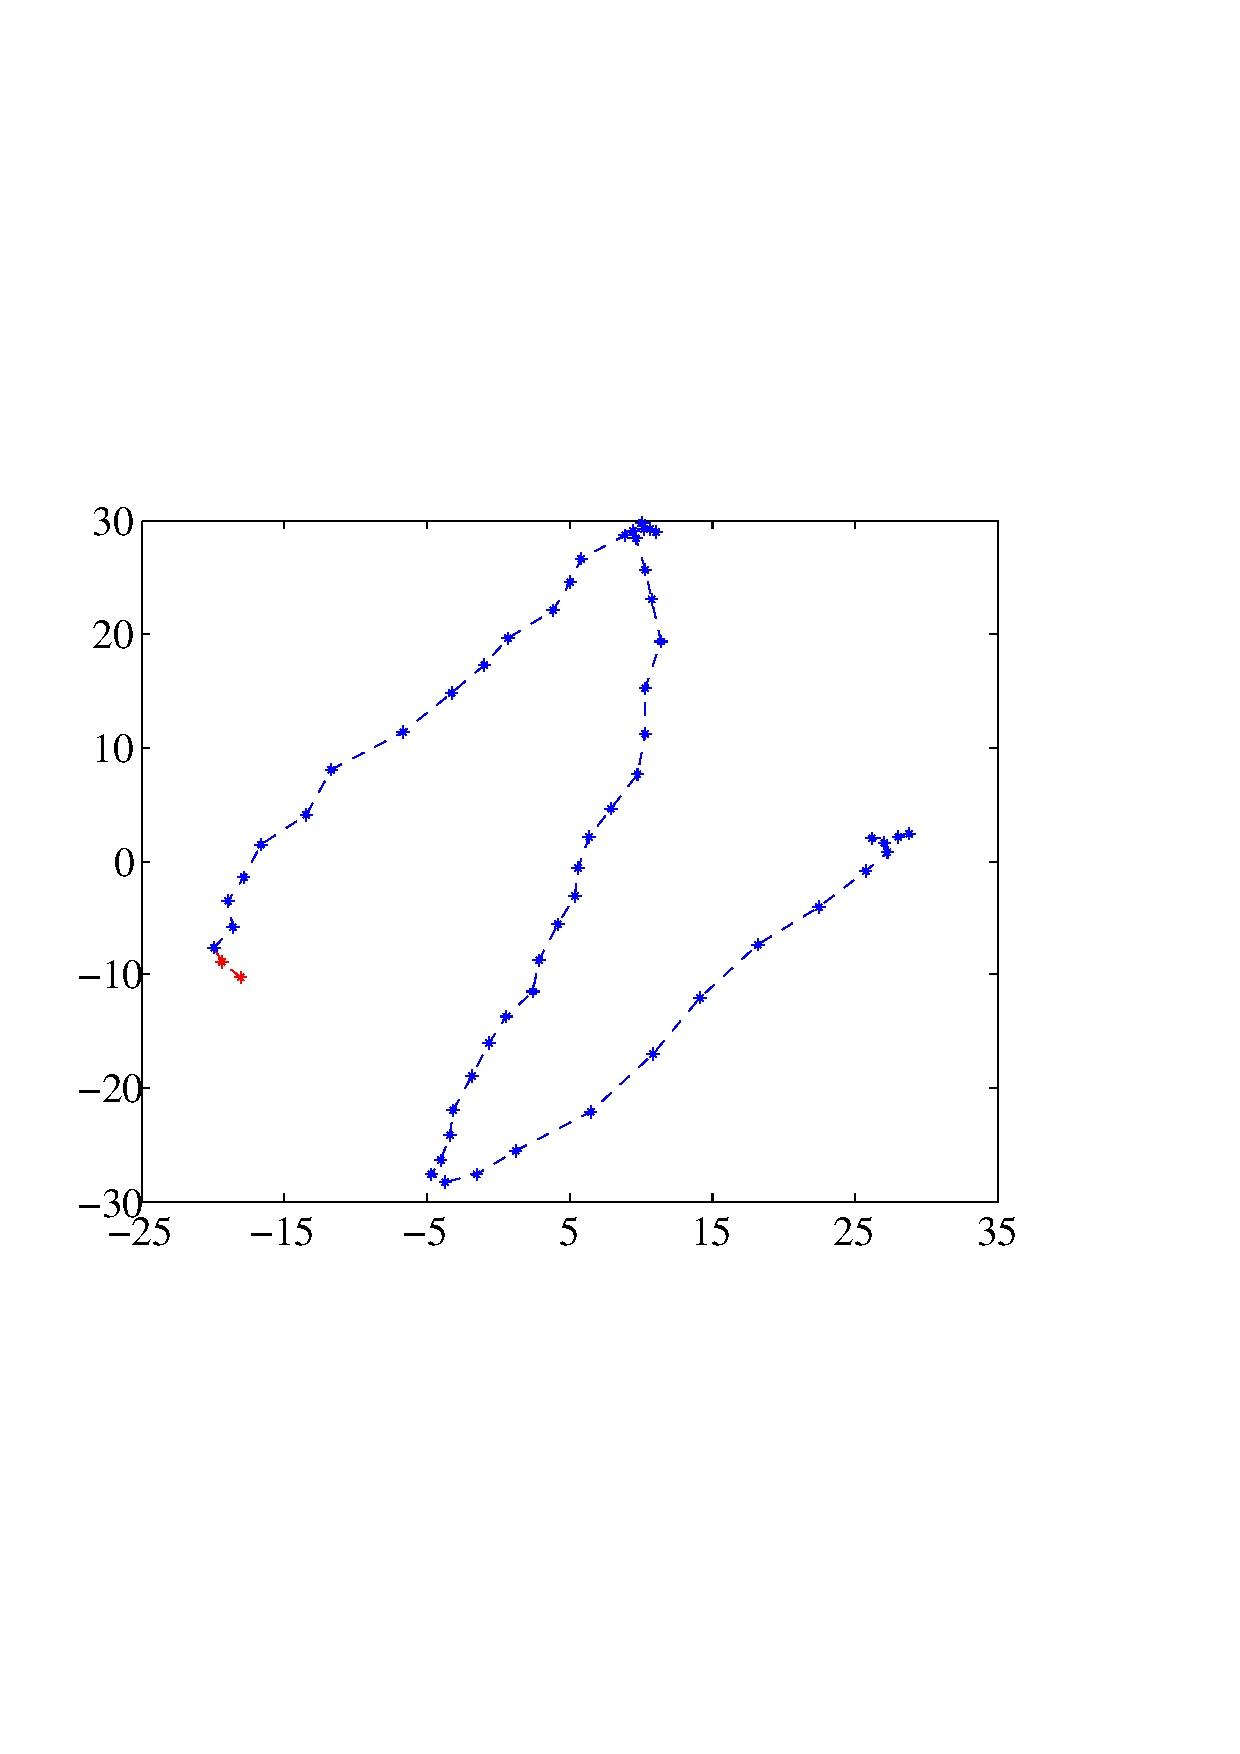
\includegraphics[width=3.8cm]{fig/distance-2m.pdf}\\
                \centering \footnotesize (a)
                \end{minipage}
            }
            \hspace{-0.1cm}
            \subfigure{
                \begin{minipage}[b]{3.8cm}
                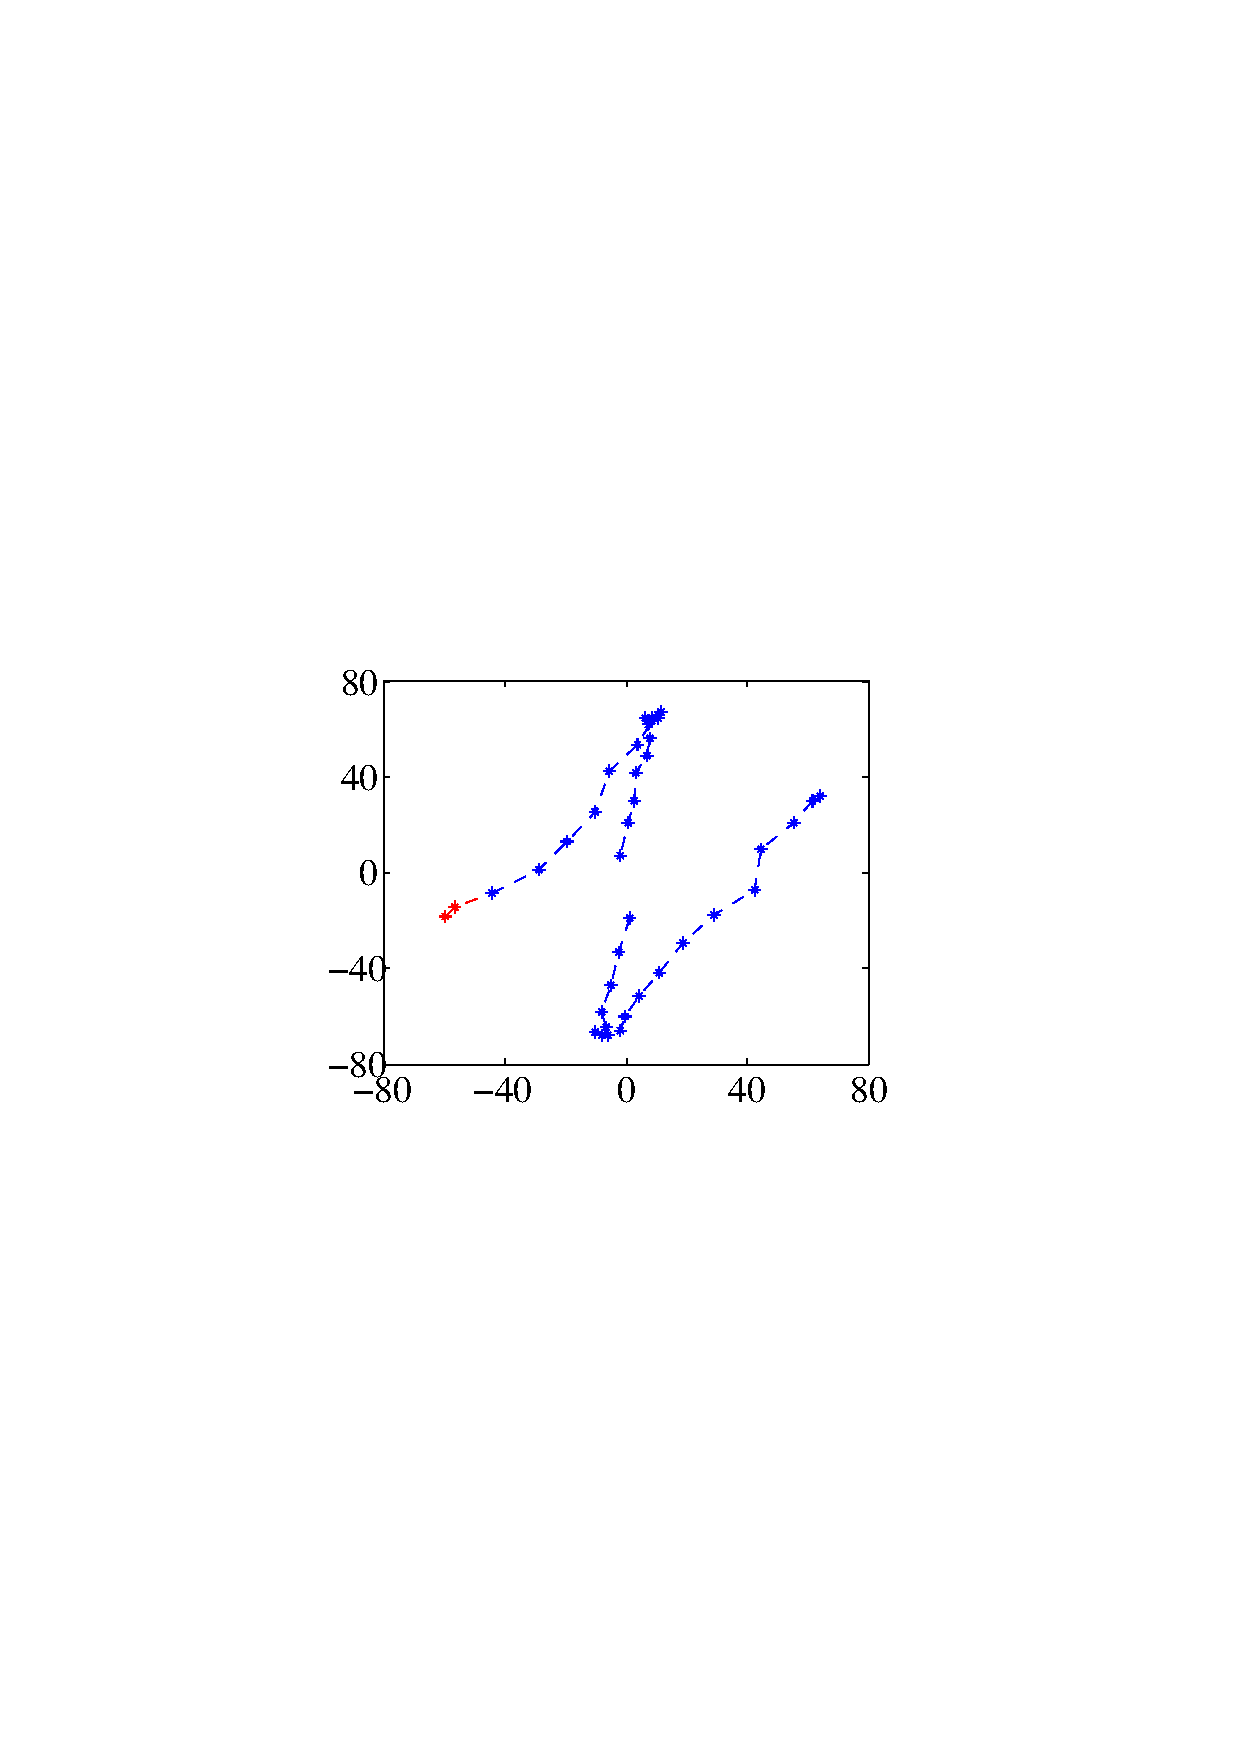
\includegraphics[width=3.8cm]{fig/distance-3m.pdf}\\
                \centering \footnotesize (b)
                \end{minipage}
            }
            \hspace{-0.1cm}
            \subfigure{
                \begin{minipage}[b]{4cm}
                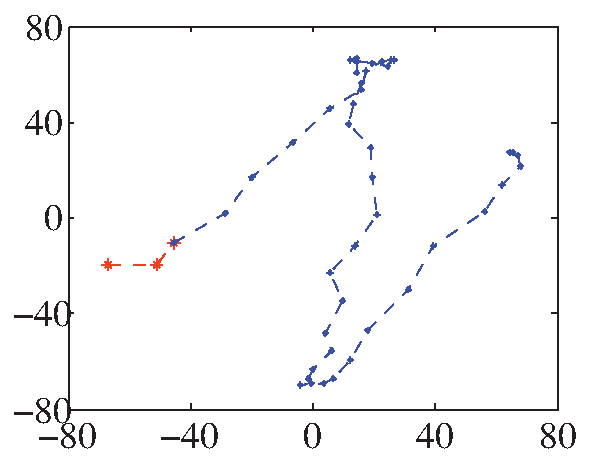
\includegraphics[width=4cm]{fig/distance-3-5m.pdf}\\
                \centering \footnotesize (c)
                \end{minipage}
            }
            \hspace{-0.1cm}
            \subfigure{
                \begin{minipage}[b]{3cm}
                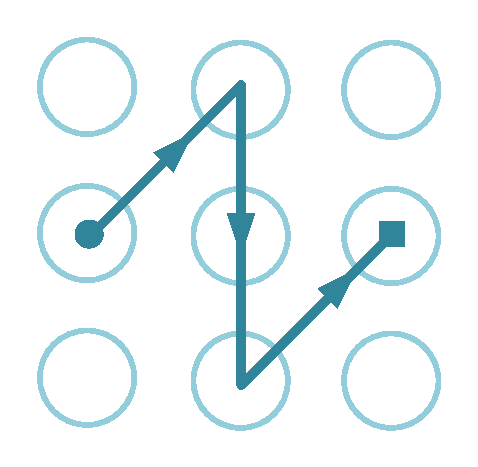
\includegraphics[width=3cm]{fig/distance-pattern.pdf}\\
                \centering \footnotesize (d)
                \end{minipage}
            }
                \vspace{-3mm}
            \caption{Tracked fingertip trajectories (user's perspective) for the pattern shown in (d) from a video filmed from a distance of 2m (a), 3m (b), and 3.5m (c) respectively away from the target device. The tracking quality decreases when the filming distance is greater than 3m. }
            \vspace{-3mm}
            \label{fig:distance-show}
        \end{figure*}



    \subsection{Impact of Filming Distances \label{sec:distances}}
        \begin{table}[!t]
            \centering
            \caption{Tracking precision vs filming distance}
            \vspace{-0.2mm}
            \label{tab:tab1}
            \small
            \begin{tabular}{ccccc}
                \toprule
                \textbf{Distance}& 1 m & 2 m & 3 m & 3.5 m \\
                \midrule
                \textbf{fingertip}  & 100\% & 98.7\% & 80.9\% & 68\% \\
                \textbf{device edge} & 100\% & 99.4\% & 90.6\% & 69\% \\
                \bottomrule
            \end{tabular}
            \vspace{-5mm}
        \end{table}


        \noindent \textbf{Result 2:} \emph{We can crack over 80\% of the patterns in five attempts, if the video was filmed using a smartphone within a distance of 2.5 meters away from the target.}

           We would like to know how the filming distance affects the
           success rate of the attack. To do so, we have asked our participants to randomly select all 120
           pattern locks and we varied the
           filming distance from 1 meter to 3.5 meters.
           Figure~\ref{fig:fig12} shows how the cracking success rate changes
           as the filming distance increases. There is slight differences in the success rate between this diagram and Figure~\ref{fig:fig10}
            because we used less patterns in this experiment.
           When the filming distance is less than 2 meters, our approach can crack all patterns in five attempts.
           The success rate drops significantly when
           the filming distance is greater than 2.5 meters.
           The quality of the video filmed by a mobile phone tends to drop significantly with many object deformations. The degradation of the video quality makes it difficult for the TLD algorithm to successfully track objects across video frames.
            This is confirmed by Table~\ref{tab:tab1}
           which shows that the tracking precision for the fingertip and the device edge drops from around 99\% to
           68\% when the filming
           distance increases from 2 meters to 3.5 meters. The increased
           tracking failures result in an increased number of missing
           points on the tracked trajectory, leading to a deteriorative performance in identifying candidate patterns.
           This can be seen from Figure~\ref{fig:distance-show} where the quality
           of tracking clearly decreases when the filming distance is greater
           than 3 meters.
           Nonetheless, our approach can
           achieve a high success rate when the filming distance within
           2.5 meters. Such a distance allows an attacker to
           record the video without raising suspicions in many day-to-day scenarios (some of these are
           described in Figure~\ref{fig:fig1}).

            We also evaluated our approach on videos filmed using a Nikon D90
            single-lens reflex (SLR) camera with a 105mm lens. The SLR camera
            was placed from a distance of 9 meters away from the target
            device. For this set of videos, we are able to achieve the same
            performance when compared to using videos filmed by a mobile
            phone camera with a 2-meter filming distance. The further filming
            distance is largely due to better video quality brought by the advanced
            SLR camera and the lens. Therefore, in practice, an attacker can
            also use a professional video recording device to launch the
            attack from a further distance.


    \subsection{Impact of Camera Shake}

    \noindent \textbf{Result 3:} \emph{Our method can tolerate a certain degree of camera shake in the hand-held mode.}

    In this experiment, we used an IPhone4S smartphone to record how a pattern is drawn on a Huawei Honor7 phone. This experiment was carried out under three settings:
    \emph{fixed}, \emph{hand-held} and \emph{shaky}, where the filming
    device was respectively fixed using a tripod, hand-held, and hand-held but with constant movements of
     approximate 2cm in the horizontal or the vertical directions. The recording device was placed on the left-front, front, and right-front of the target device.
    In the experiment, we fixed the target device on a table using double-sided tapes.

    We use a reference point to quantify camera shake. The point
    is the center position of an area of the target device. The area is marked by a boundary box on the first
    frame (see Figure~\ref{fig:fig5}). We calculate the difference (in terms of pixels) for where the
    reference point was seen in two consecutive video frames. We then use the difference to measure the degree of camera shake.
    Figure~\ref{fig:fig13} shows the cumulative distribution function (CDF)
    of camera shake under the three different filming settings.
    Here, the wider the distribution is, the less steady the
     filming is. The shaky mode is least stable where the difference of the reference point between two video frames can be up to 250 pixels.


    Figure~\ref{fig:fig14} shows that our approach has the same performance under
    the hand-held and the fixed modes. The modest camera sake under the hand-held mode
    has little impact on performance thanks to our camera-shake-calibration method. We observe deteriorative performance
    under the shaky mode, but the performance degradation is modest (80\% vs 97\%
    in 5 attempts). In reality, an attacker would avoid drastic
    camera shake by firmly holding the video recording device.

        \begin{figure}[t!]
            \centering
            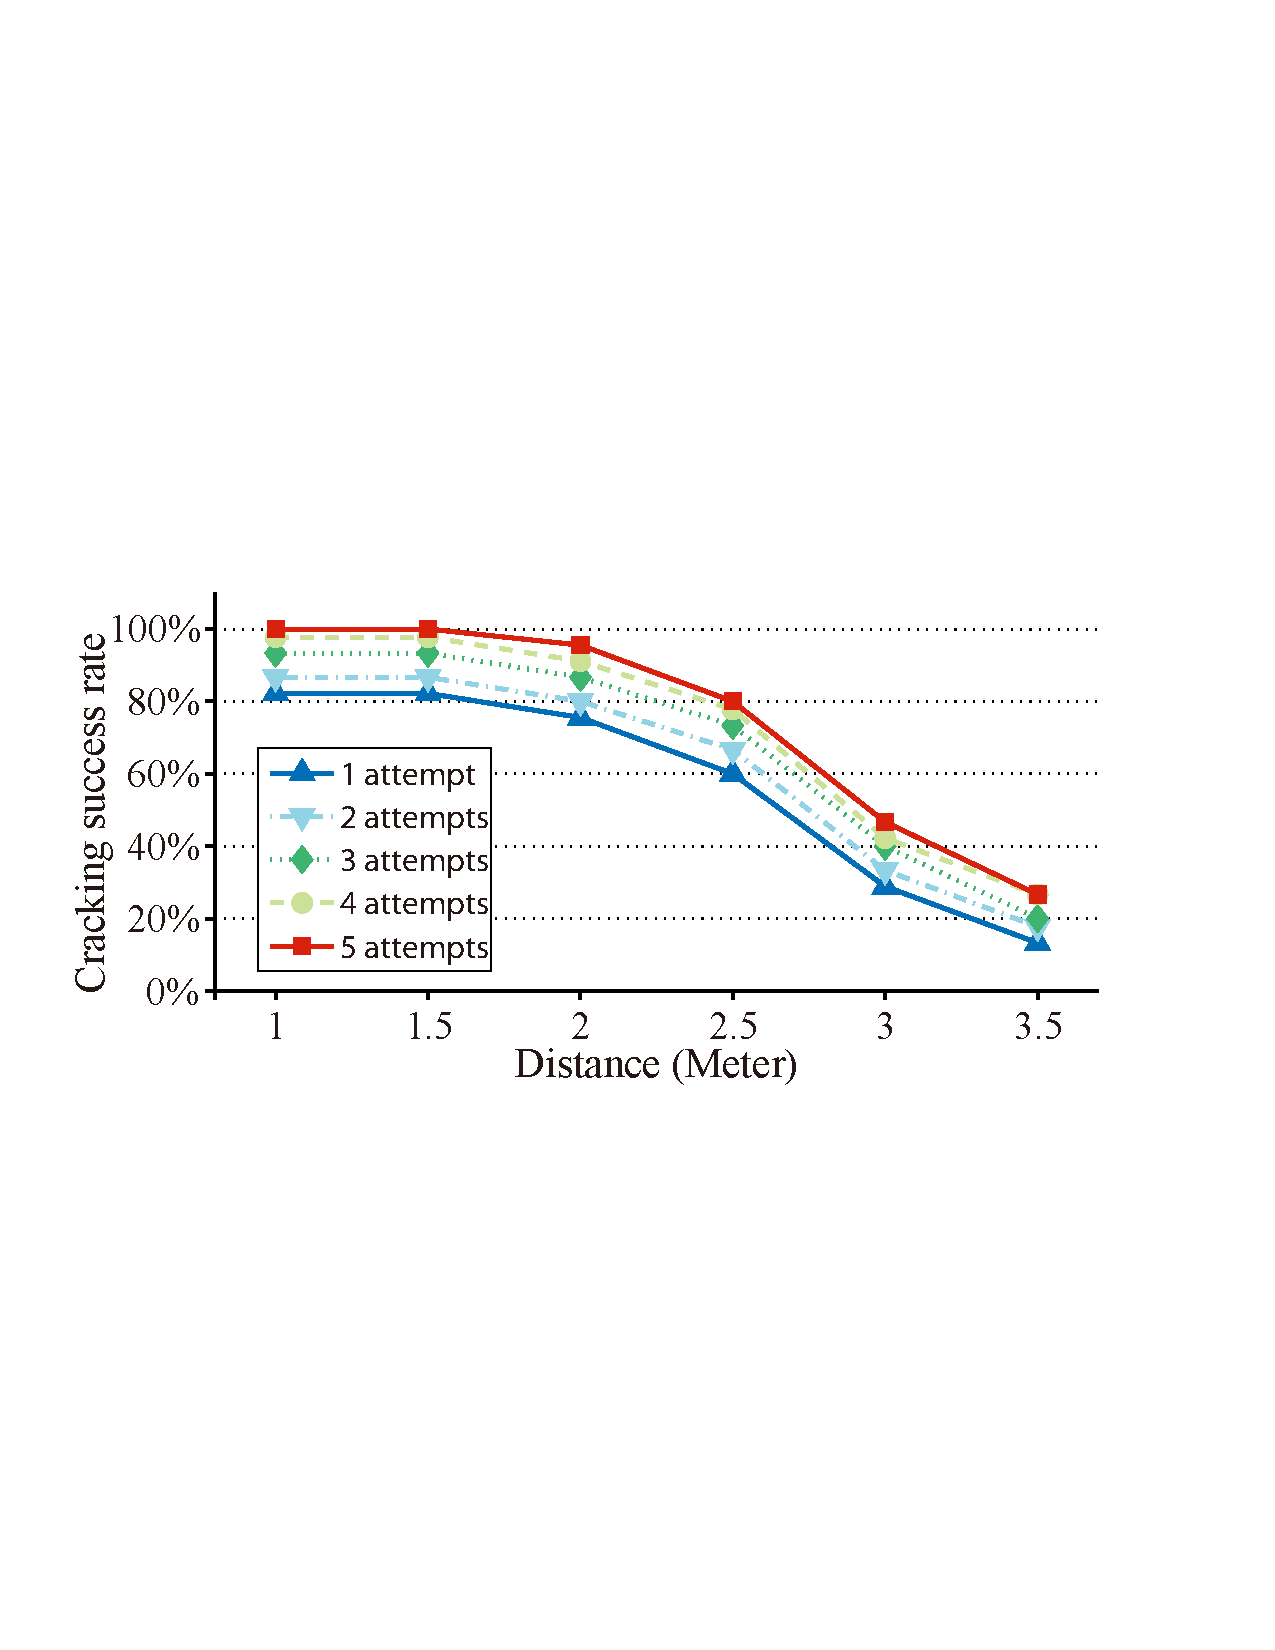
\includegraphics[width=0.35\textwidth]{fig/12.pdf}
            \vspace{-3mm}
            \caption{Impact of the filming distance.}
            \label{fig:fig12}
           \vspace{-3mm}
        \end{figure}

\begin{figure}[t!]
    \centering
    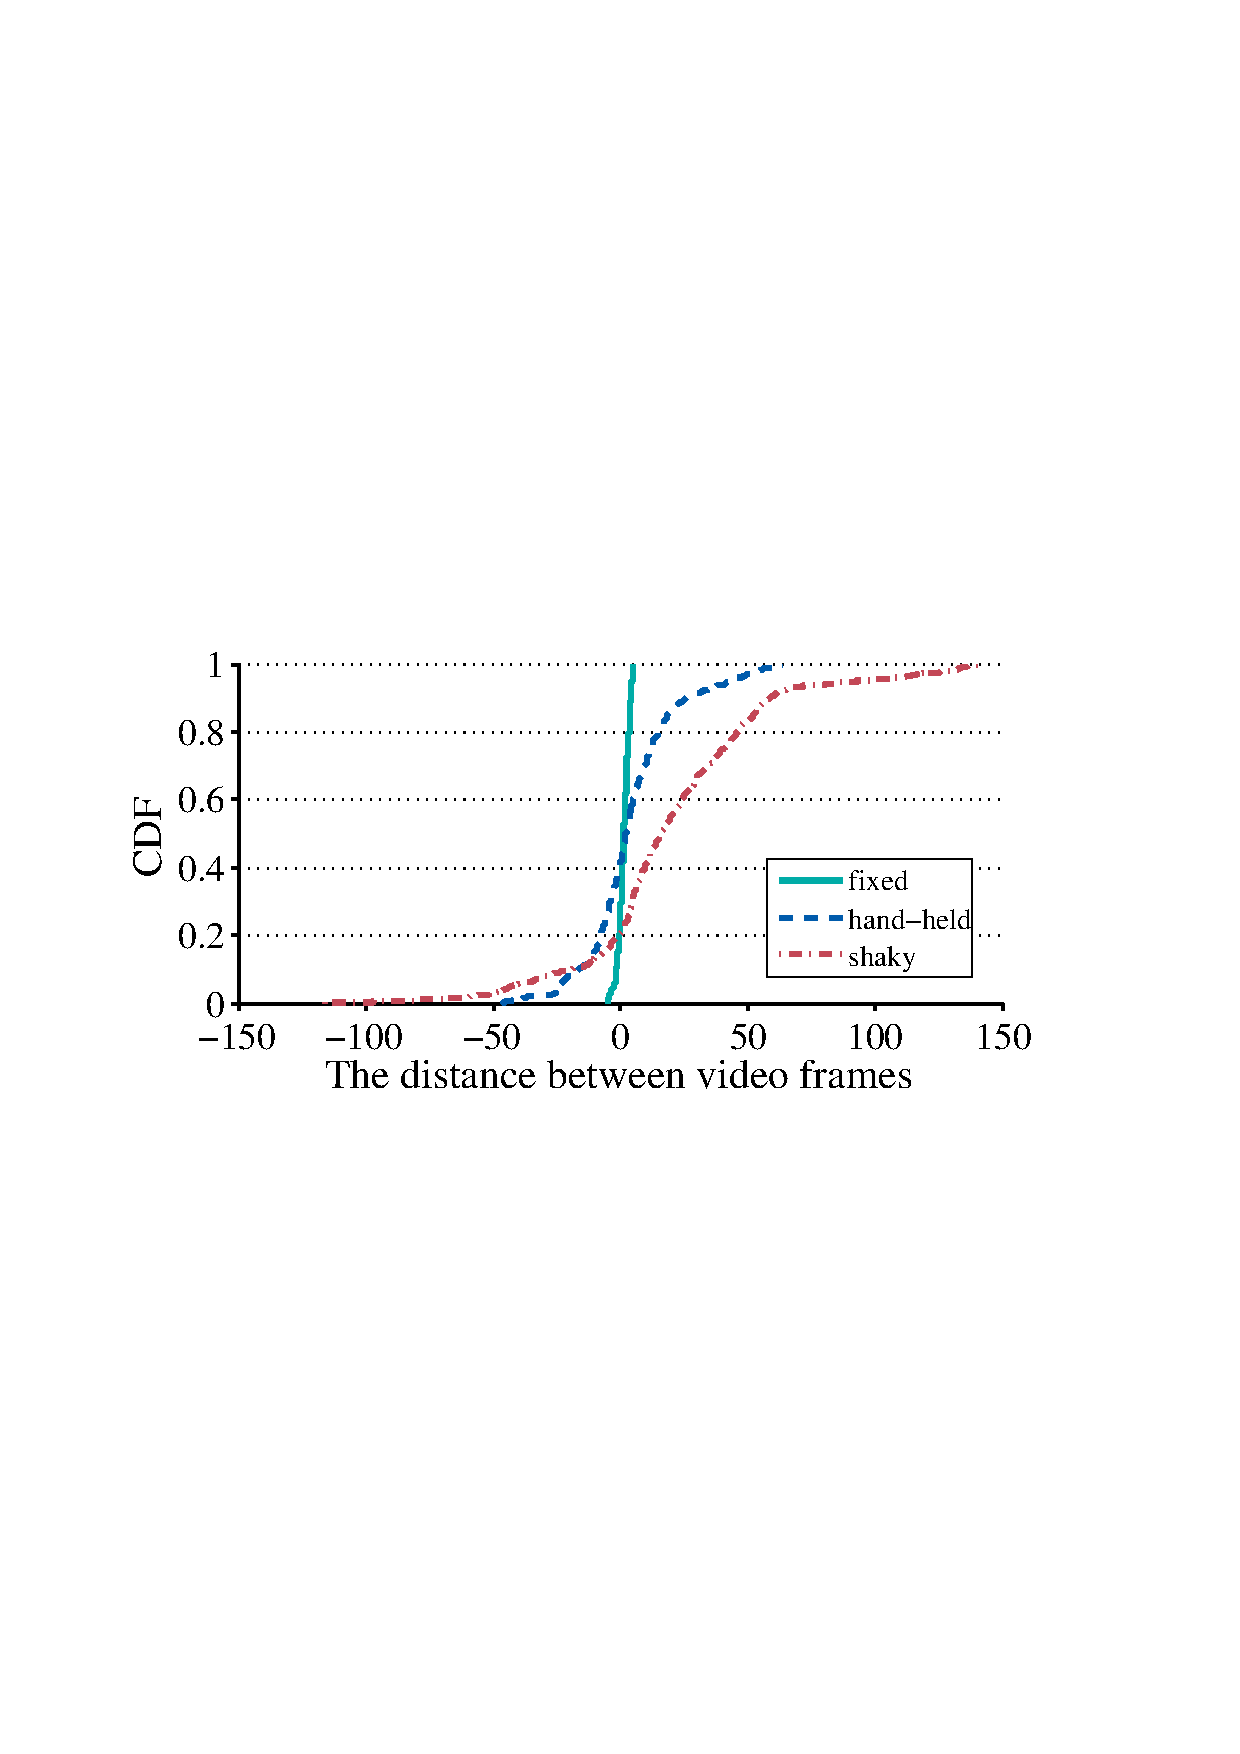
\includegraphics[width=0.35\textwidth]{fig/13.pdf}
    \vspace{-2mm}
    \caption{The cumulative distribution function (CDF) for different video recording modes.}
    \vspace{-2mm}
    \label{fig:fig13}
\end{figure}

\begin{figure}[!t]
    \centering
    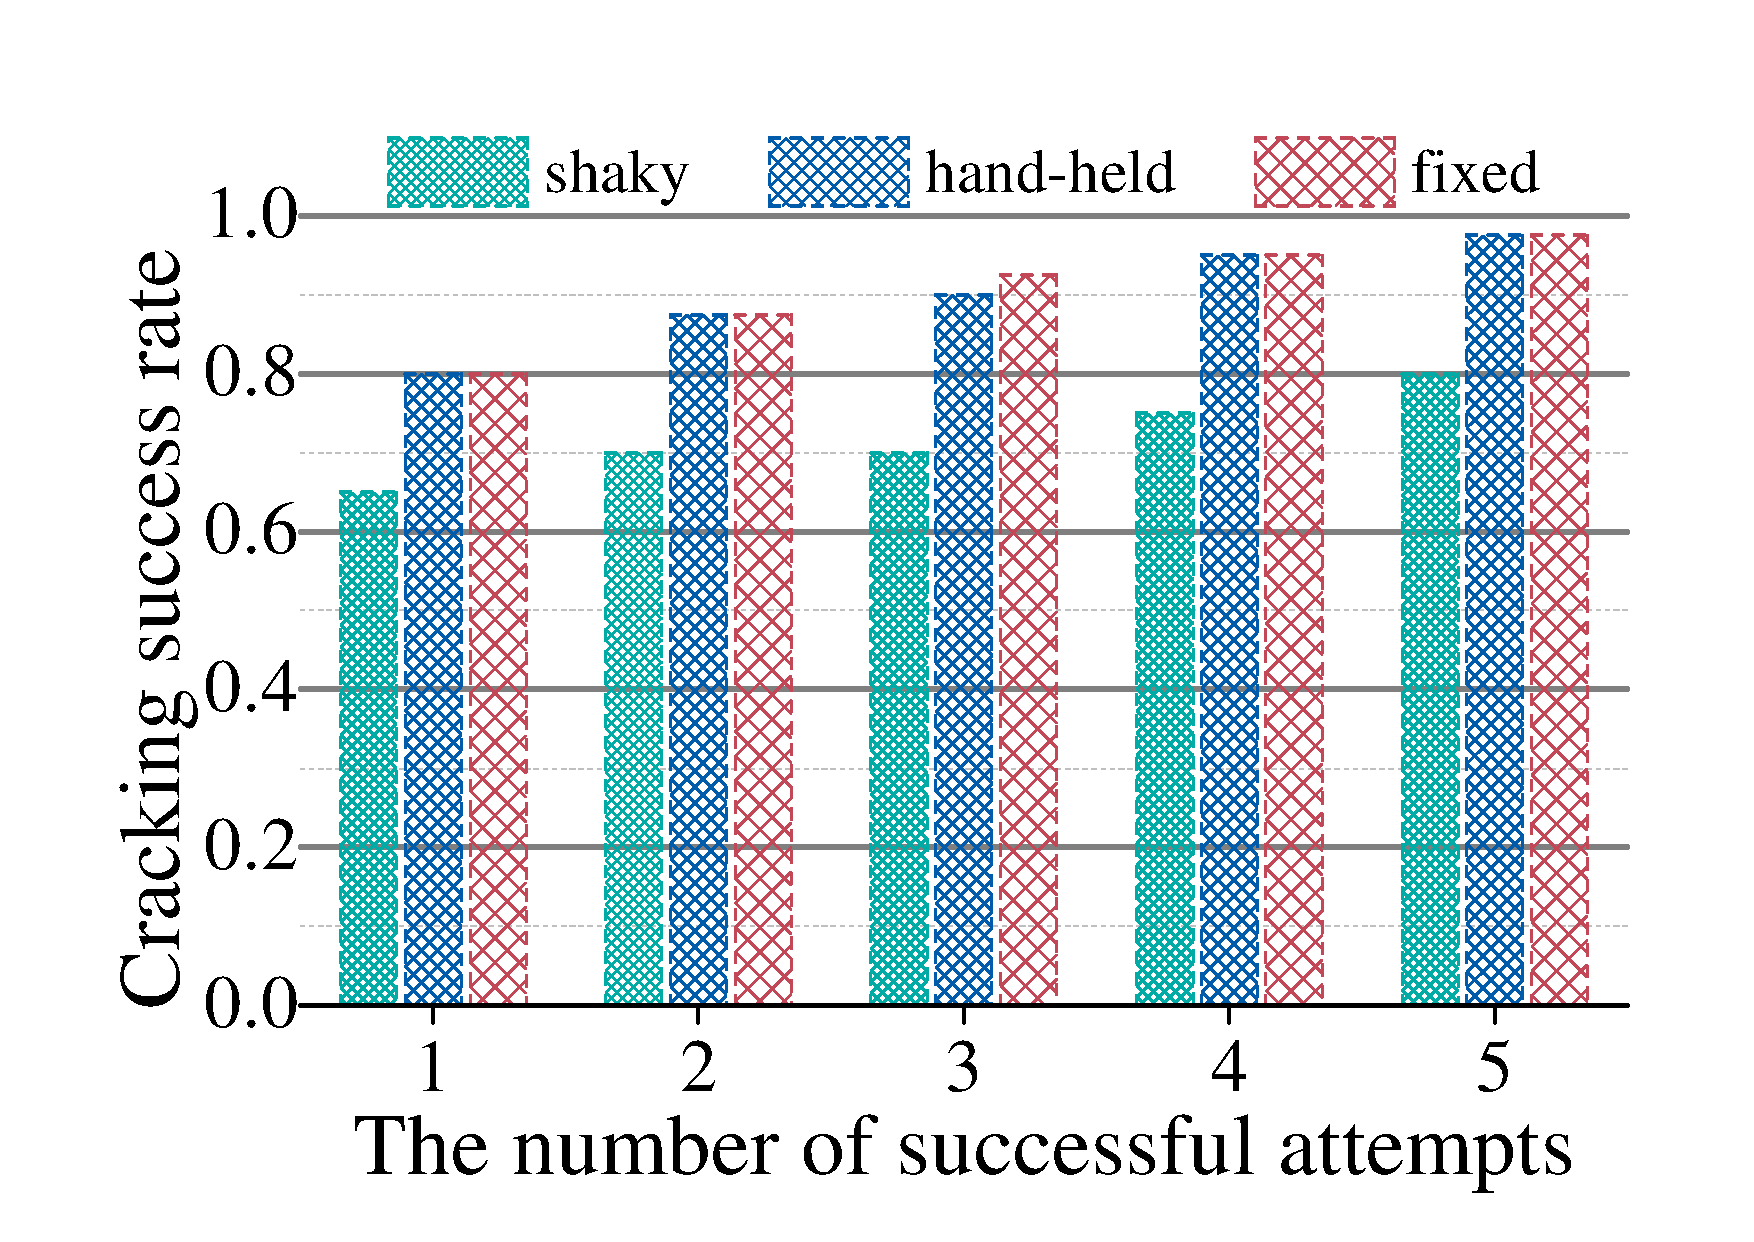
\includegraphics[width=0.35\textwidth]{fig/14.pdf}
    \vspace{-2mm}
    \caption{Impact of camera shake. Our approach has the same success rate under the hand-held and the fixed modes and the performance degradation under the shaky mode is modest. }
    %\FIXME{We should evaluate this on 3 and 4 attempts.}
   \vspace{-2mm}
    \label{fig:fig14}
\end{figure}





    \subsection{Impact of Lighting Conditions \label{sec:light}}
    \noindent \textbf{Result 4:} \emph{Low-light has a negative impact on the success rate of the attack but our approach can still break over 70\% of the patterns when the video was filmed in a low-light environment.}

    In this experiment, videos were recorded under different lighting conditions both indoor and outdoor.
    The experimental settings are given in  Table~\ref{tab:light}.
    The light intensity of these condidtions ranges from 9500
    lux (strong light), onto 240 lux (normal light), and 55-70 lux (low light).
    These represent some of the day-to-day scenarios where filming can
    take place. For each setting, we asked each of our 10 participants to draw all collected 120 patterns on a Xiaomi MI4 phone. We used
    an iPhone4S phone to record the video. The filming camera was place on the
    left-front, front, and the right-front of the target device from a distance
    of 2 meters.


    Figure~\ref{fig:light} shows that the success rate increases when video filming were performed in a brighter lighting condition as the light intensity
    changes from 55 lux to 9500 lux. This is expected as low-light leads to
    increased video noise, blurred motion and poor focus, which all have a
    negative impact on the TLD algorithm. Nonetheless, our attack
    can still crack over 70\% of the patterns in a filming
    environment with low light.

            \begin{table}[!t]
            \centering
            \caption{Lighting Conditions}
            \label{tab:light}
            \scriptsize
            \begin{tabular}{lcccc}
                \toprule
                \textbf{Scenarios} & Indoor  & Indoor & Indoor  & Outdoor\\
                \midrule
                \textbf{Time} & nighttime &  nighttime & daytime & daytime \\
                \textbf{Light Source}& warm LED & white fluorescent & sunlight &  sunlight \\
                \textbf{Light Intensity (Lux)} & $55-70$ & $70-100$ & $150$--$240$ & $500$--$9500$ \\
                \bottomrule
            \end{tabular}
            \vspace{-2mm}
        \end{table}


       \begin{figure}[t!]
            \centering
            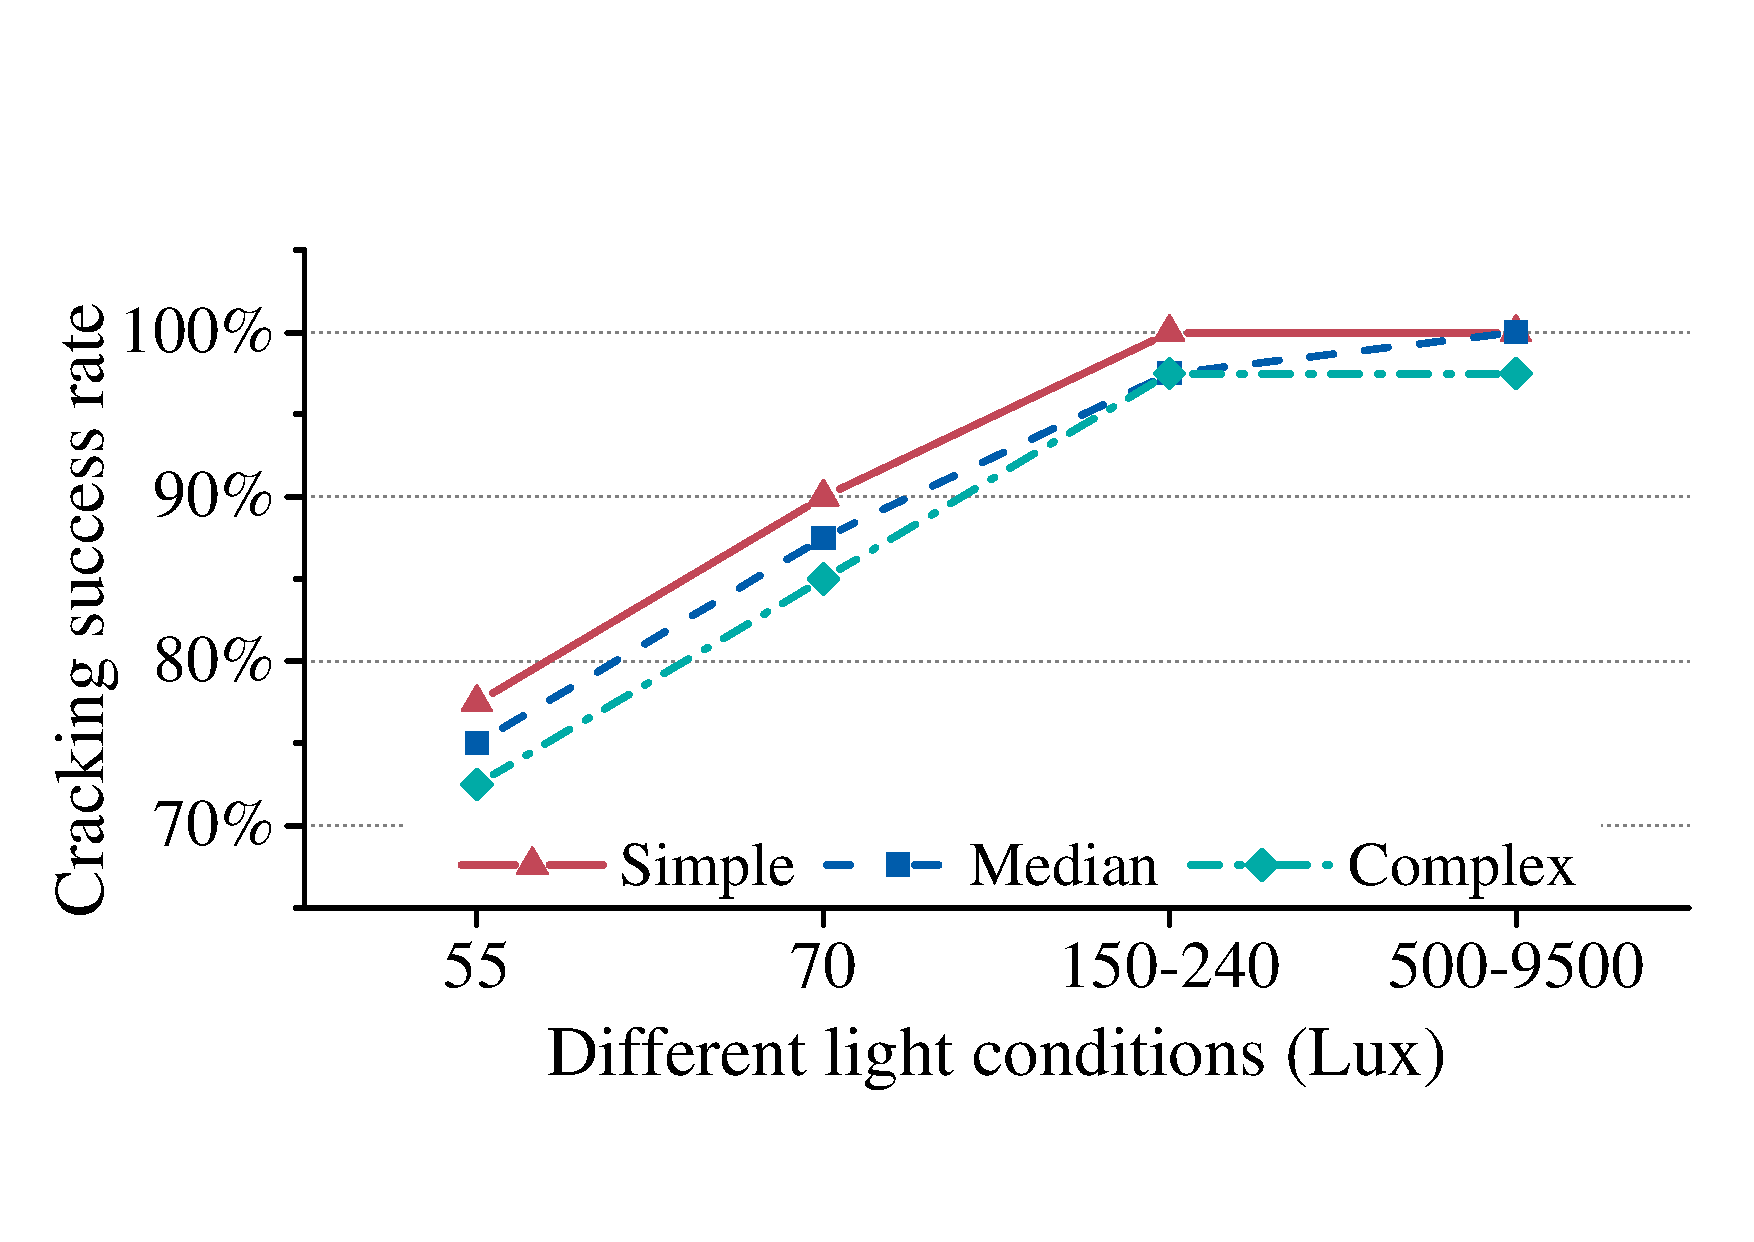
\includegraphics[width=0.35\textwidth]{fig/light.pdf}
            \vspace{-2mm}
            \caption{The cracking success rate within five attempts under different lighting conditions.}
            \label{fig:light}
        \end{figure}



    \subsection{Impact of Filming Angle Estimation \label{sec:angle}}
    \begin{figure}[!t]
        \centering
        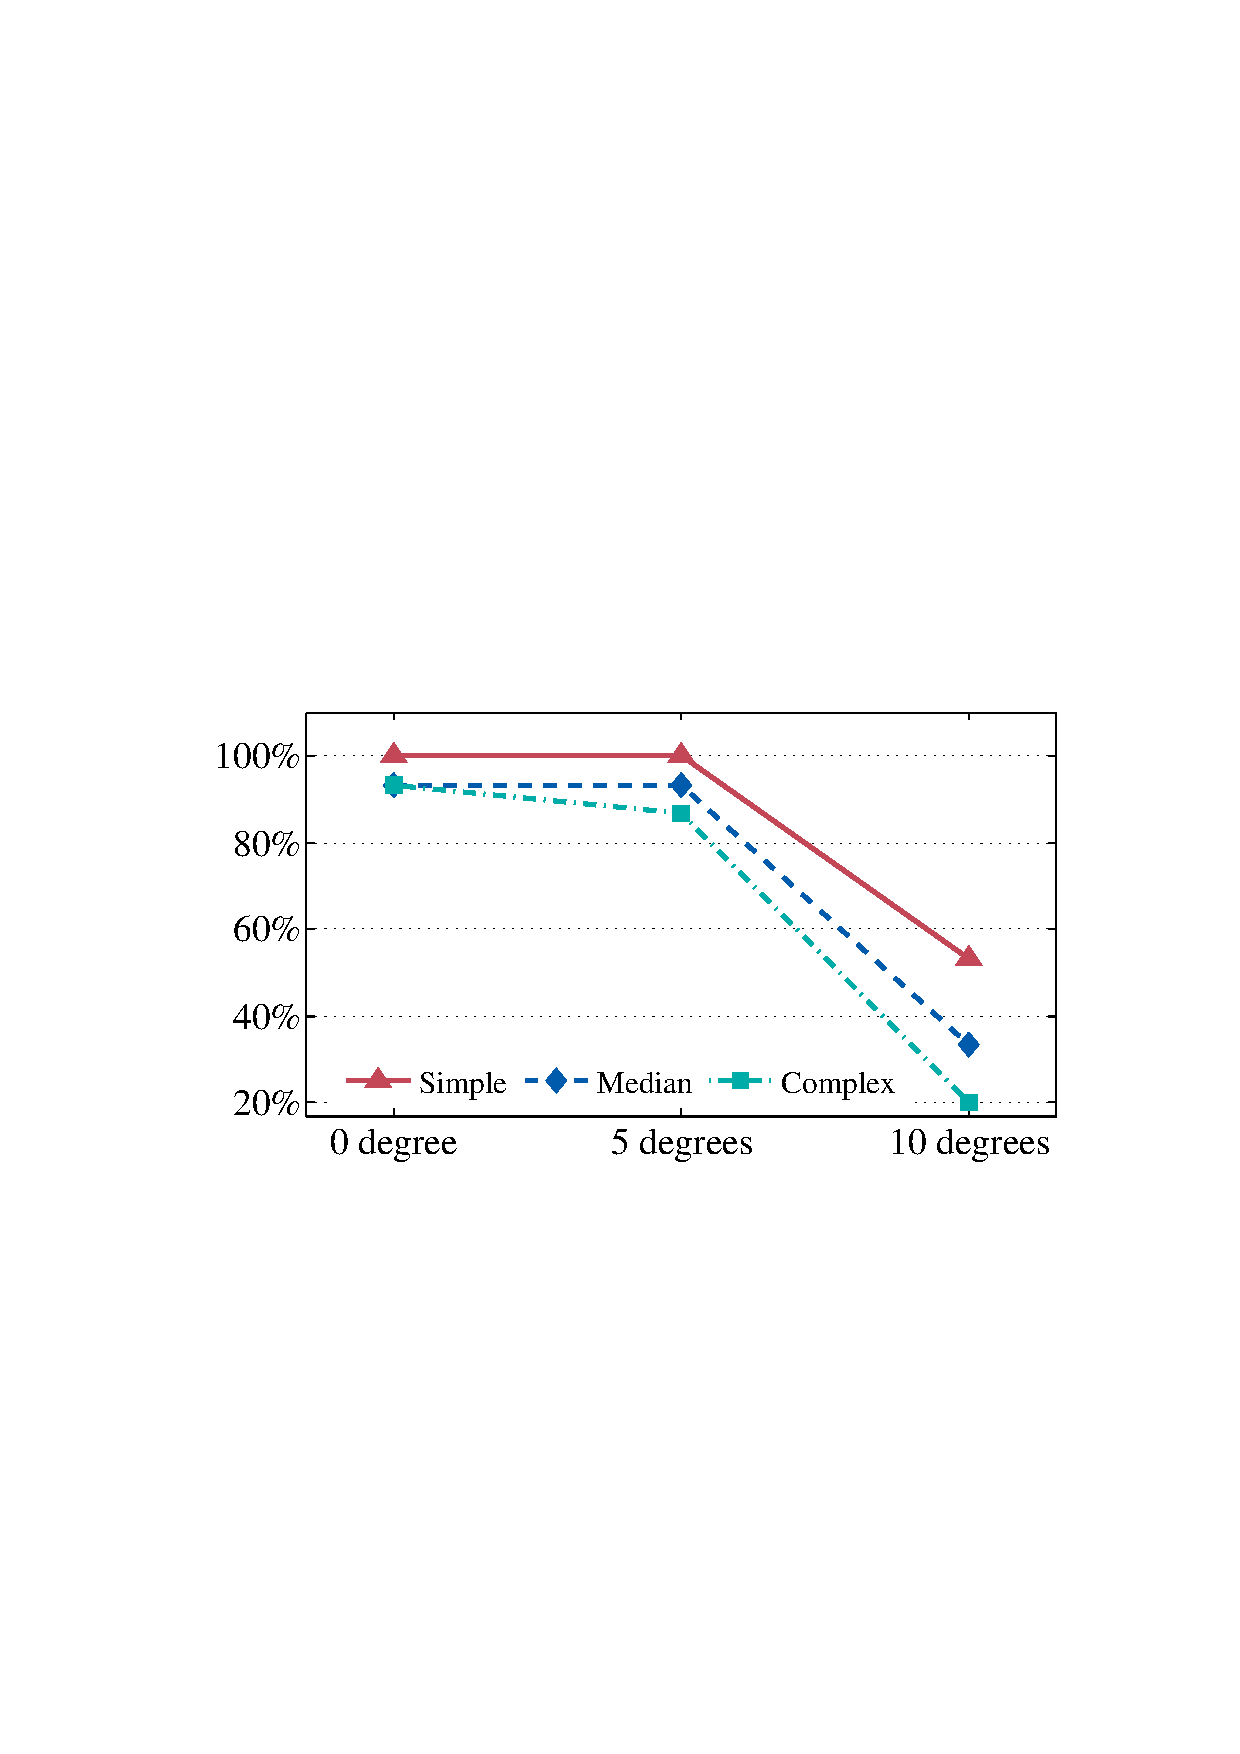
\includegraphics[width=0.35\textwidth]{fig/15.pdf}
        \vspace{-2mm}
        \caption{Impact of estimation errors of filming angles.}
        \vspace{-2mm}
        \label{fig:fig15}
    \end{figure}

    \noindent \textbf{Result 5:} \emph{Our attack performs well when the error of filming angle estimation is less than 5 degrees.}

   Our approach needs to transform the tracked fingertip movement trajectory to the
   user's perspective based on an estimation of the filming angle
   (Section~\ref{sec:transformation}).
   Because our filming angle estimation
    algorithm gives highly accurate estimation, we did not find the estimation error to be a problem in our experiments.
   Nonetheless, it is worth studying how the estimation error affects the success rate of our attack. To do so, we deliberately added an error of 5-10 degrees to the estimation.

    Figure~\ref{fig:fig15} shows the results of this experiment. When the error is less than $\pm 5$ degrees, there is little impact
    on \emph{complex} patterns and no impact at all on \emph{simple} and
    \emph{median} patterns. However, an estimation error of more than 10 degrees can significantly affect the success rate.
    Given such an error, the resulted trajectory after transformations will
    be significant different from the correct pattern.
    For example, when the estimation error is 10 degrees from the
    true value,  on average, 0.8, 2.6 and 4.2 line segments per pattern respectively will
    be incorrectly labelled for \emph{simple}, \emph{median} and
    \emph{complex} patterns. This explains why the success rate for complex patterns drops significantly when there is
    an error of 10 degrees.

    \subsection{\FIXED{Impact of Different Targets and Cameras}}
    \noindent \textbf{Result 6:} \emph{The size of smartphone touch-screen and brands of mobile camera had little effect on the success rate.}

    Intuitively, the success rate may be influenced by the size of touch-screen because the length of pattern will be short as the screen size decreases. Likewise, the accuracy also may be influenced by the quality of video as the different quality of phone cameras. To evaluate this effection, we ask 10 participants to randomly select 60 patterns (30 patterns for each category). We use IPhone6, Xiaomi MI4, Vivo X7, Samsung Note4 to record unlock videos while the patterns are drawn on IPhone4S\footnote{Participants draw patterns on the login interface of Alipay installed on the phone as Apple operating system do not support pattern lock authentication mechanism.}, Huawei Honor7 and Samsung Galaxy Tab E. The distance is 2m away from the tester during record the unlocking process. Table~\ref{tab:screen-size} shows the sizes of screen vary from 3.5\emph{inch} (IPhone4S) to 9.6\emph{inch} (Samsung Tab) which involve almost all screen size of smart devices used in daily life.
    Table~\ref{tab:camera-parameters} presents the mobile cameras and their main parameters used in this experiment. The parameters for the four mobile cameras have few differences and these differences determine the function of the cameras in specific shooting scenes. For example, Note4 camera have a longer focal length than other three mobile camera, which means that its effective shooting distance is longer than others. We believe that the four mobile cameras represent the most common cameras used by people of all walks of life.

    Figure~\ref{fig:screen_size} (a) shows our approach has the same performance under different sizes of phone screens. We observe the success rate reach 98.3\% within five attempts when the screen size is 3.5\emph{inch}, the smallest screen on the mobile market, and our method can crack all tested pattern locks when the size of screen is larger than 5.2\emph{inch} (Honor7). We also evaluated the our approach using different types of phone cameras for filming videos. The result is presented in Figure~\ref{fig:screen_size} (b). Our method can reconstruct all patterns within five trials using IPhone6 and Note4 cameras because they are able to capture high quality videos. Anyway, the success rate can reach 96.7\% and 98.3\% within five attempts respectively using MI4 and Vivo X7 cameras. This prove that our method perfects well with common used phone cameras.

    \begin{table}[!t]
            \centering
            \caption{Touch-screen sizes for the test phones}
            \label{tab:screen-size}
            \scriptsize
            \begin{tabular}{|c|c|c|c|}
                \hline
                \diagbox[dir=SE]{Size}{Brands}& IPhone4S & Honor7 & Samsung Tab \\
                \hline
                Height(cm)$\times$Width(cm) & $11.5\times5.9$ & $14.3\times7.2$ & $24.2\times15.0$ \\
                \hline
            \end{tabular}
            %\vspace{-4mm}
    \end{table}

    \begin{table}[!t]
            \centering
            \caption{The main parameters for the phone camera}
            \label{tab:camera-parameters}
            \small
            \begin{tabular}{|c|c|c|c|c|}
                \hline
                \diagbox[dir=SE]{Parm}{Brands}& IPhone6 & Vivo X7 & MI4 & Note4 \\
                \hline
                Frame Rate (fps) & $30$ & $30$& $30$ & 30 \\
                \hline
                Pixels & 8mp & 13mp & 13mp & 16mp \\
                \hline
                Focus (mm) & 4.15 & 4 & 4 & 4.2 \\
                \hline
                Sensitivity (ISO) & 3200 & 3200 & 3000 & 5000 \\
                \hline
            \end{tabular}
    \end{table}

    \begin{figure}[!t]
        \centering
        \subfigure{
             \begin{minipage}[t]{0.4\textwidth}
                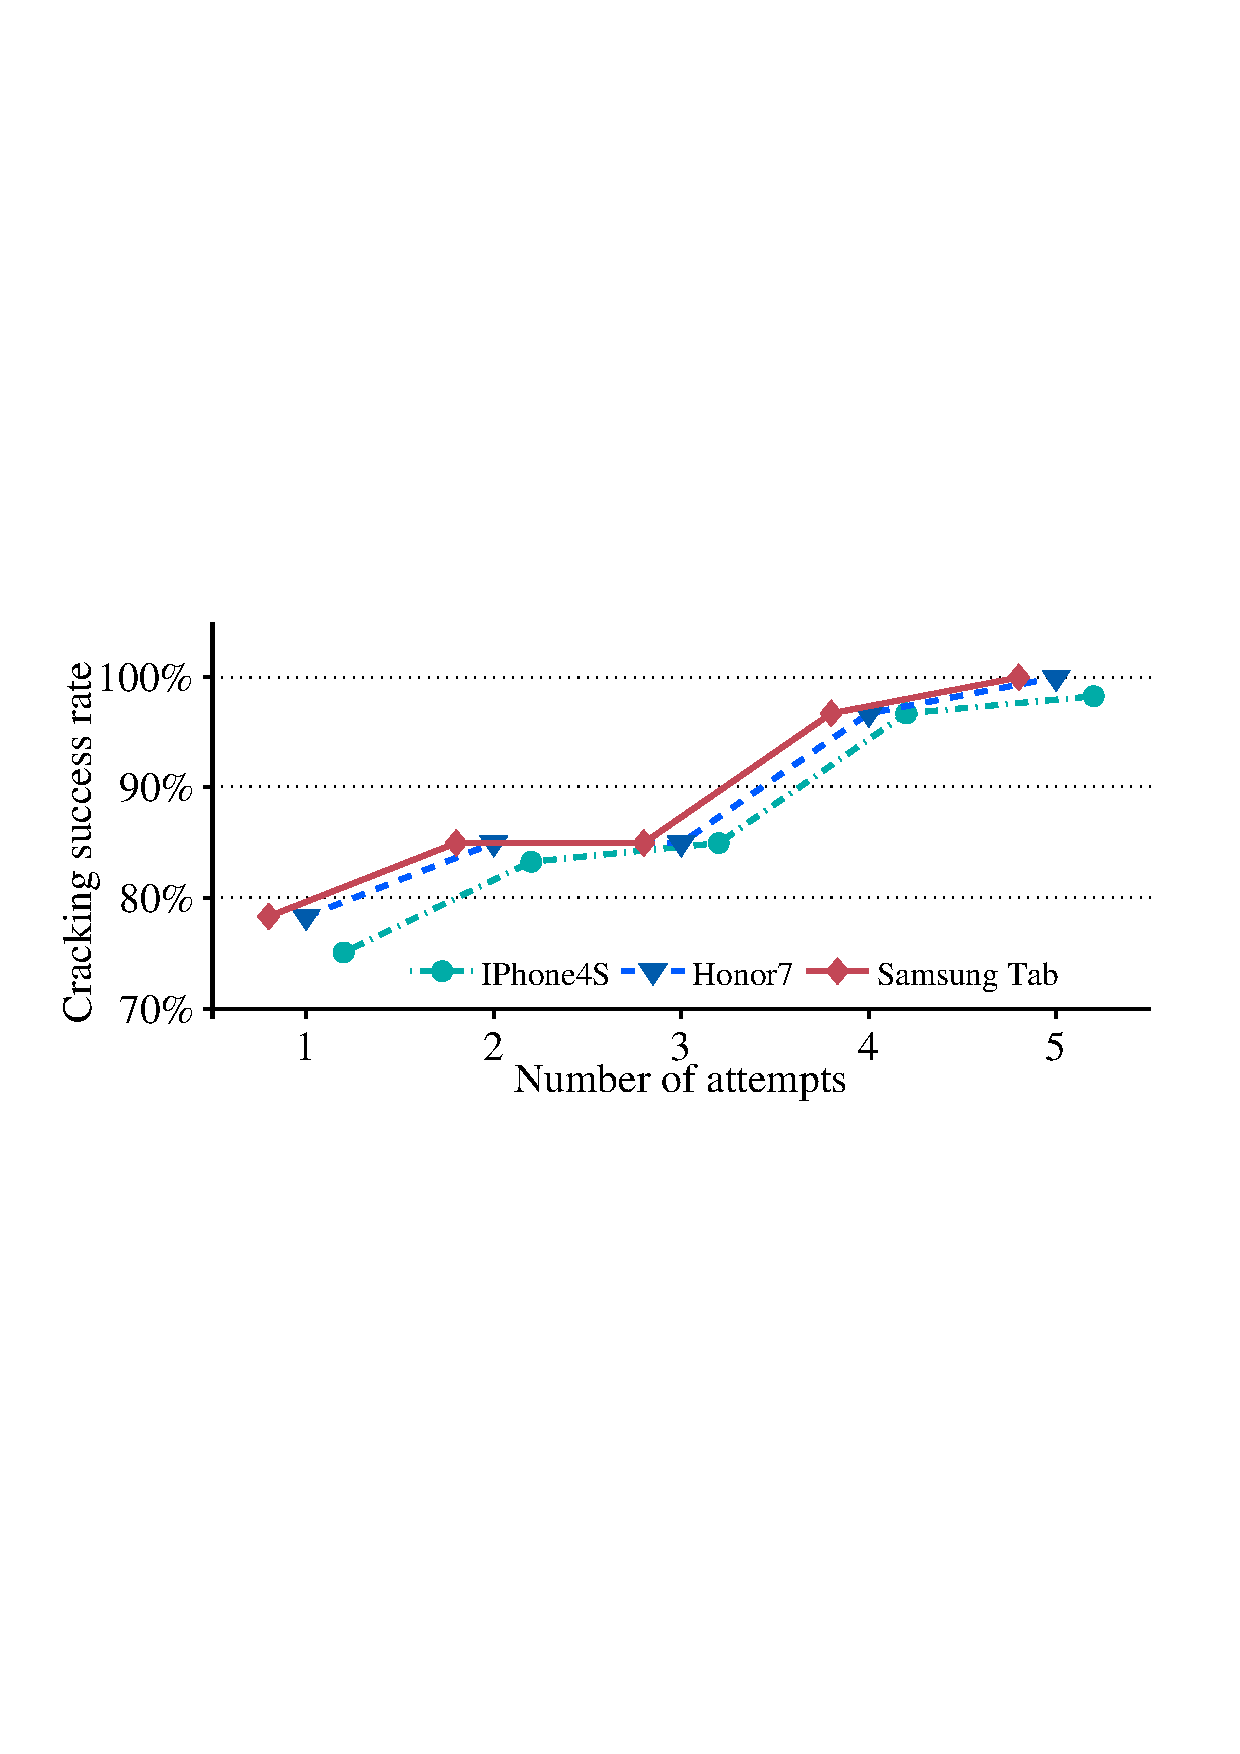
\includegraphics[width=\textwidth]{fig/screen_size.pdf}\\
                \centering \footnotesize (a) screen size
             \end{minipage}
        }
        \subfigure{
             \begin{minipage}[t]{0.4\textwidth}
                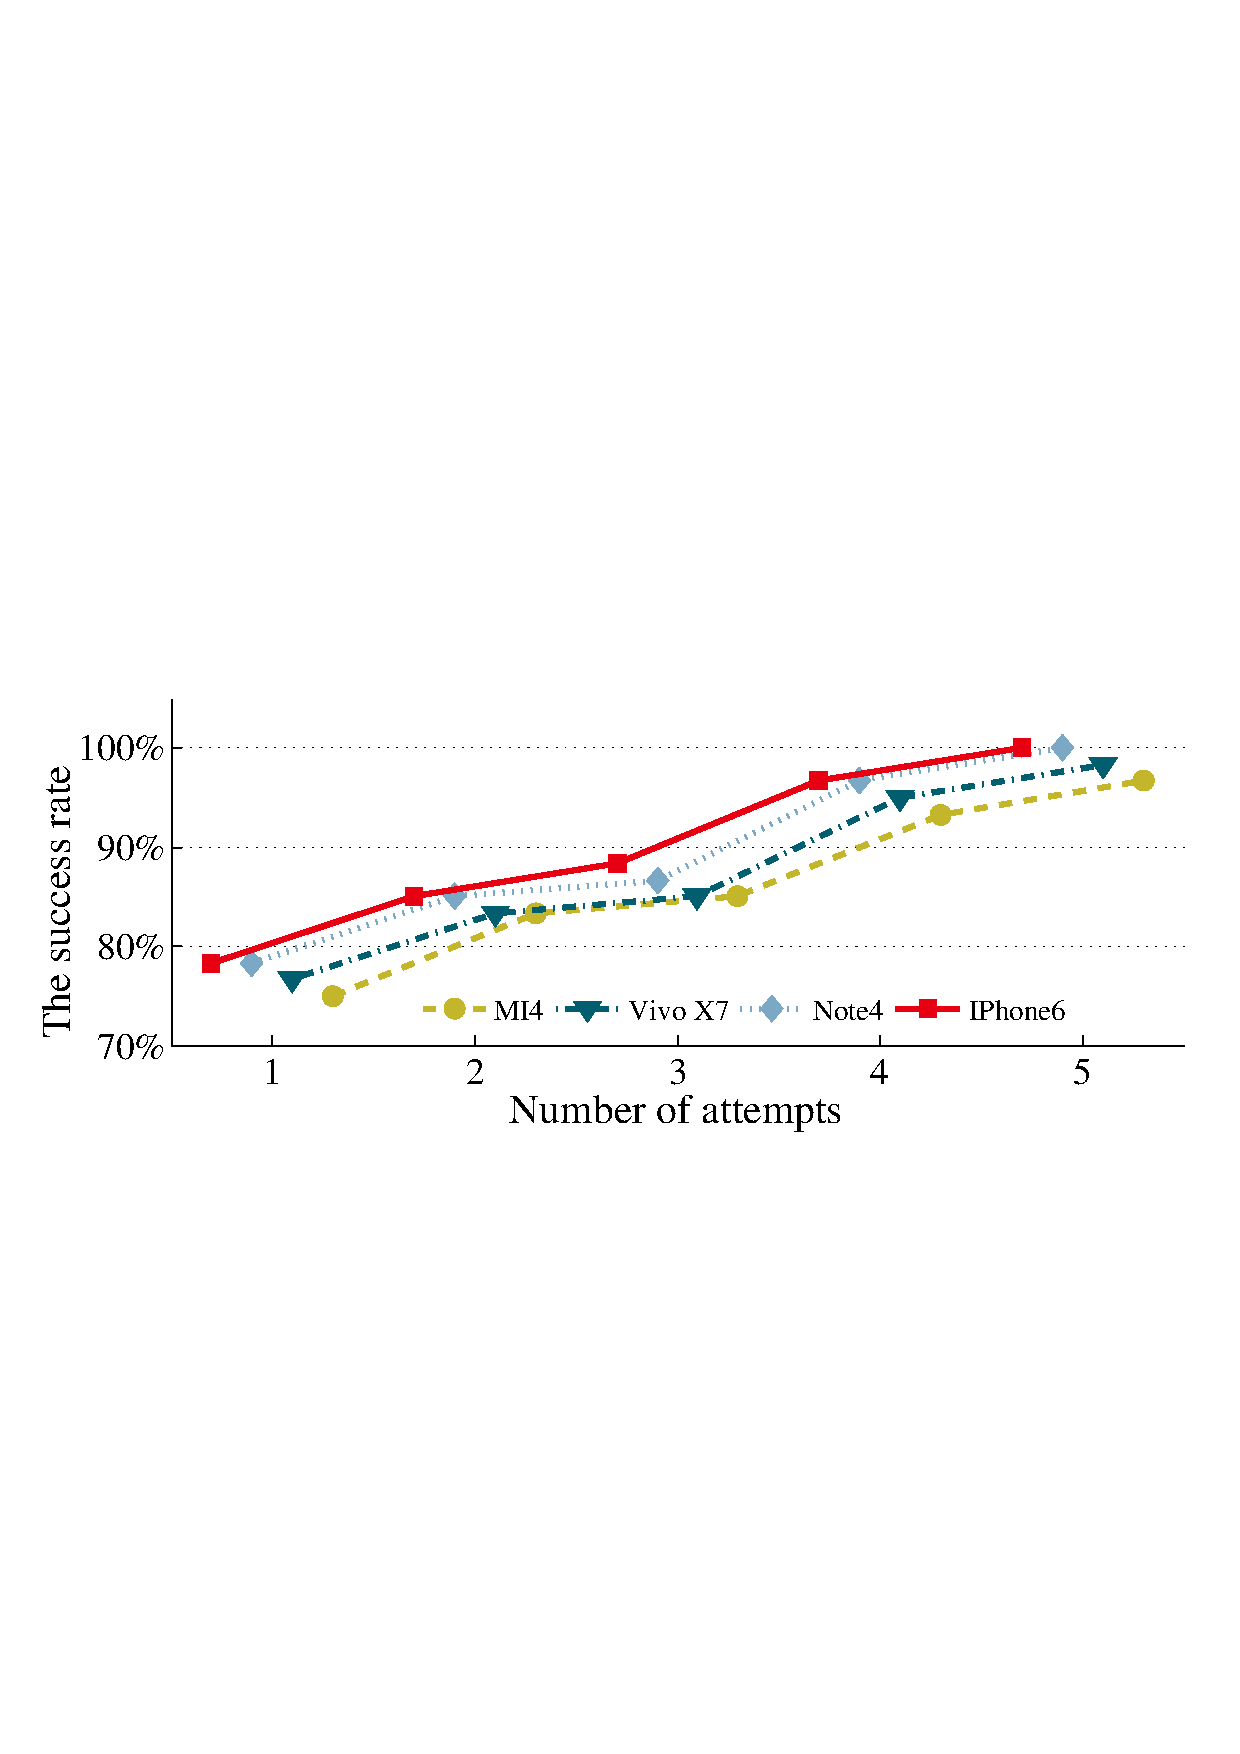
\includegraphics[width=\textwidth]{fig/camera_brands.pdf}\\
                \centering \footnotesize (b) camera brands
             \end{minipage}
        }
        \caption{The cracking success rate under different screen size and brands of camera. The difference in horizontal axis is for the purpose of illustration.}
        \label{fig:screen_size}
    \end{figure}

    \subsection{Inferring Patterns with Eyes}

    \noindent \textbf{Result 7:} \emph{Our attacking methodology significantly outperform direct observation techniques.}

   In this experiment, we investigate whether an attacker can infer the pattern by
   simply watching the video or through direct observations. To answer this question, we asked each of our 10 participants to watch 60 videos (where
   a pattern was drawn by other participants) to guess the pattern.  We
    only played the video segment during which a pattern is drawn to the participant (around 3 seconds per video).
   To familiarize participants with the process, we
    played  five sample videos and showed the correct patterns at the end of each video to our participants before the experiment.
   Each participant then had 10 minutes to watch a video and five chances to guess a pattern. They could adjust the playing speed and
   replay the video multiple times as they wished.


        Figure~\ref{fig:look-unlocking process} (a) shows the success rate of pattern guessing with
        bare eyes. Our participants correctly guessed for nearly half of the
        simple patterns in five attempts. However, they found that it is difficult
        to infer complex patterns with many line segments, overlapping lines and intersections.
        The success rate of guessing complex patterns is less than 10\% in five attempts.
        This is not a surprising result
        because although it is possible to correctly guess patterns with
        simple structures by watching the video, doing so for patterns with
        more complex structures is much harder.


    We also asked participants to directly observe how a pattern was drawn
    from a distance of 2 meters away from the target device. The intuition
    behind this evaluation is that human eyes can catch richer information
    over a video camera. The results of this experiment are shown in
    Figure~\ref{fig:look-unlocking process} (b).  As can be seen from the
    diagram, although the success rate is improved compared to directly watching the video, the chances for guessing the correct pattern in
    5 attempts are quite low. In
    fact, the success rates are just 48.3\%, 38.3\%
    and 11.7\% respectively for simple, median and complex patterns.

        \begin{figure}[!t]
            \centering
            \subfigure{
                \begin{minipage}[t]{0.35\textwidth}
                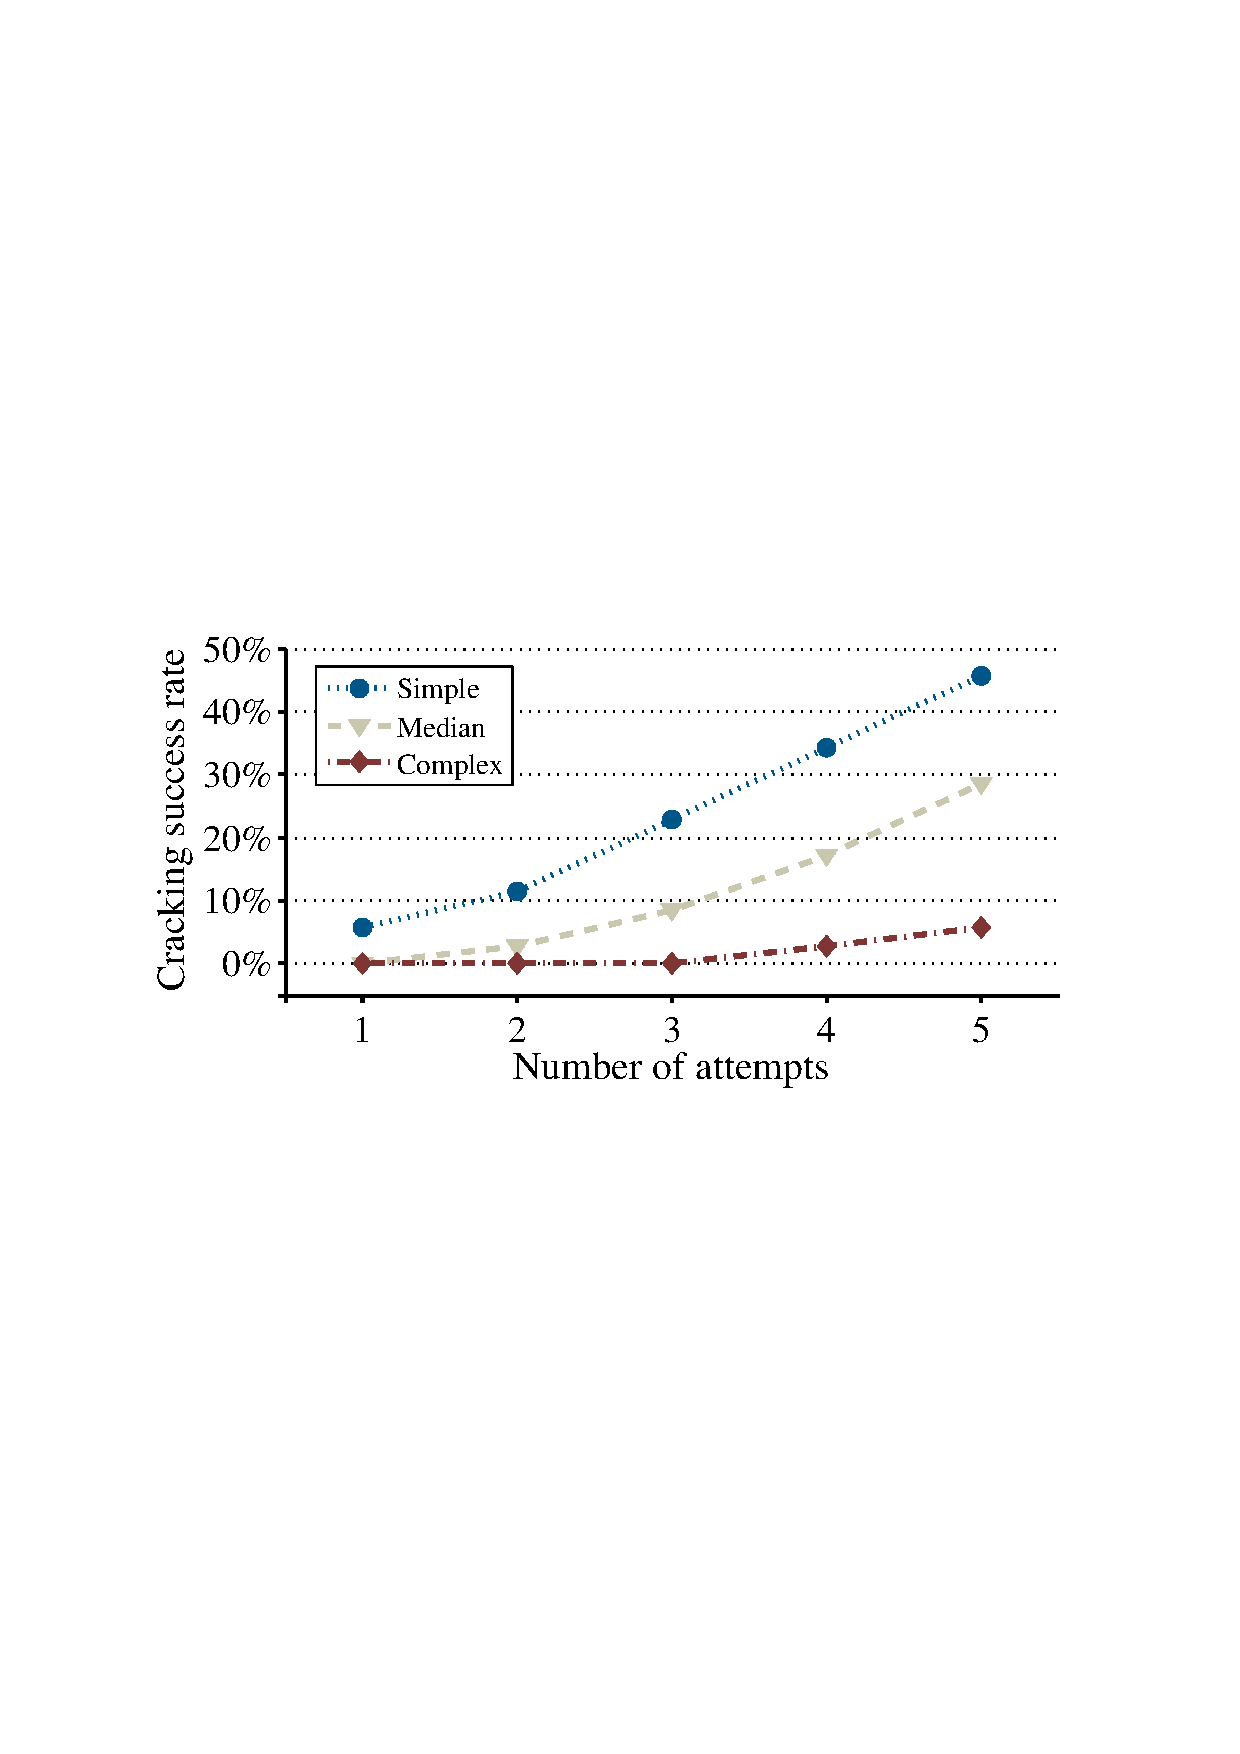
\includegraphics[width=\textwidth]{fig/look-video.pdf}\\
                \centering \footnotesize (a) video watching
                \end{minipage}
            }
            \hspace{-0.1cm}
            \subfigure{
                \begin{minipage}[t]{0.35\textwidth}
                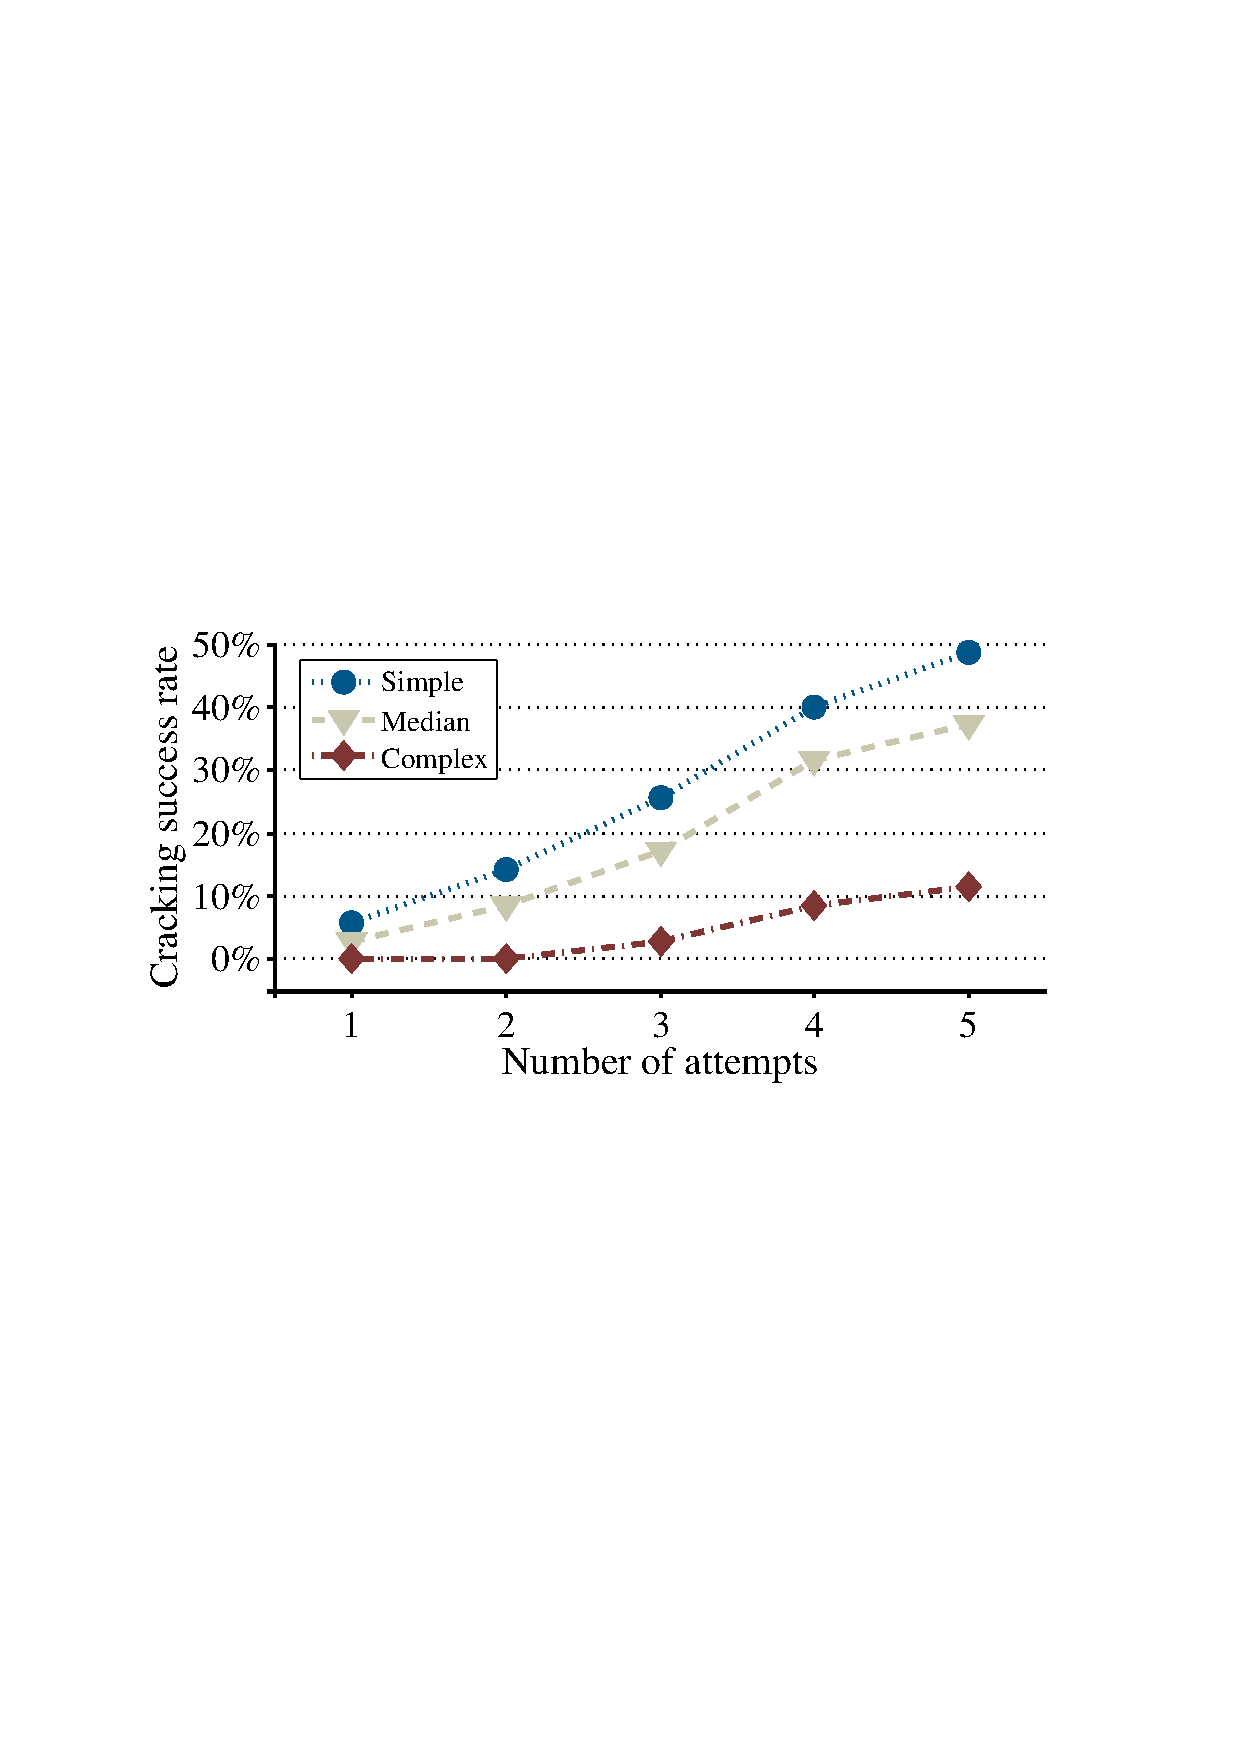
\includegraphics[width=\textwidth]{fig/look-finger.pdf}\\
                \centering \footnotesize (b) direct observations
                \end{minipage}
            }
            \vspace{-2mm}
            \caption{Success rates of guessing patterns through watching the video (a) or direct observations (b).}
            \label{fig:look-unlocking process}
        \end{figure}

        \begin{figure}[!t]
            \centering
            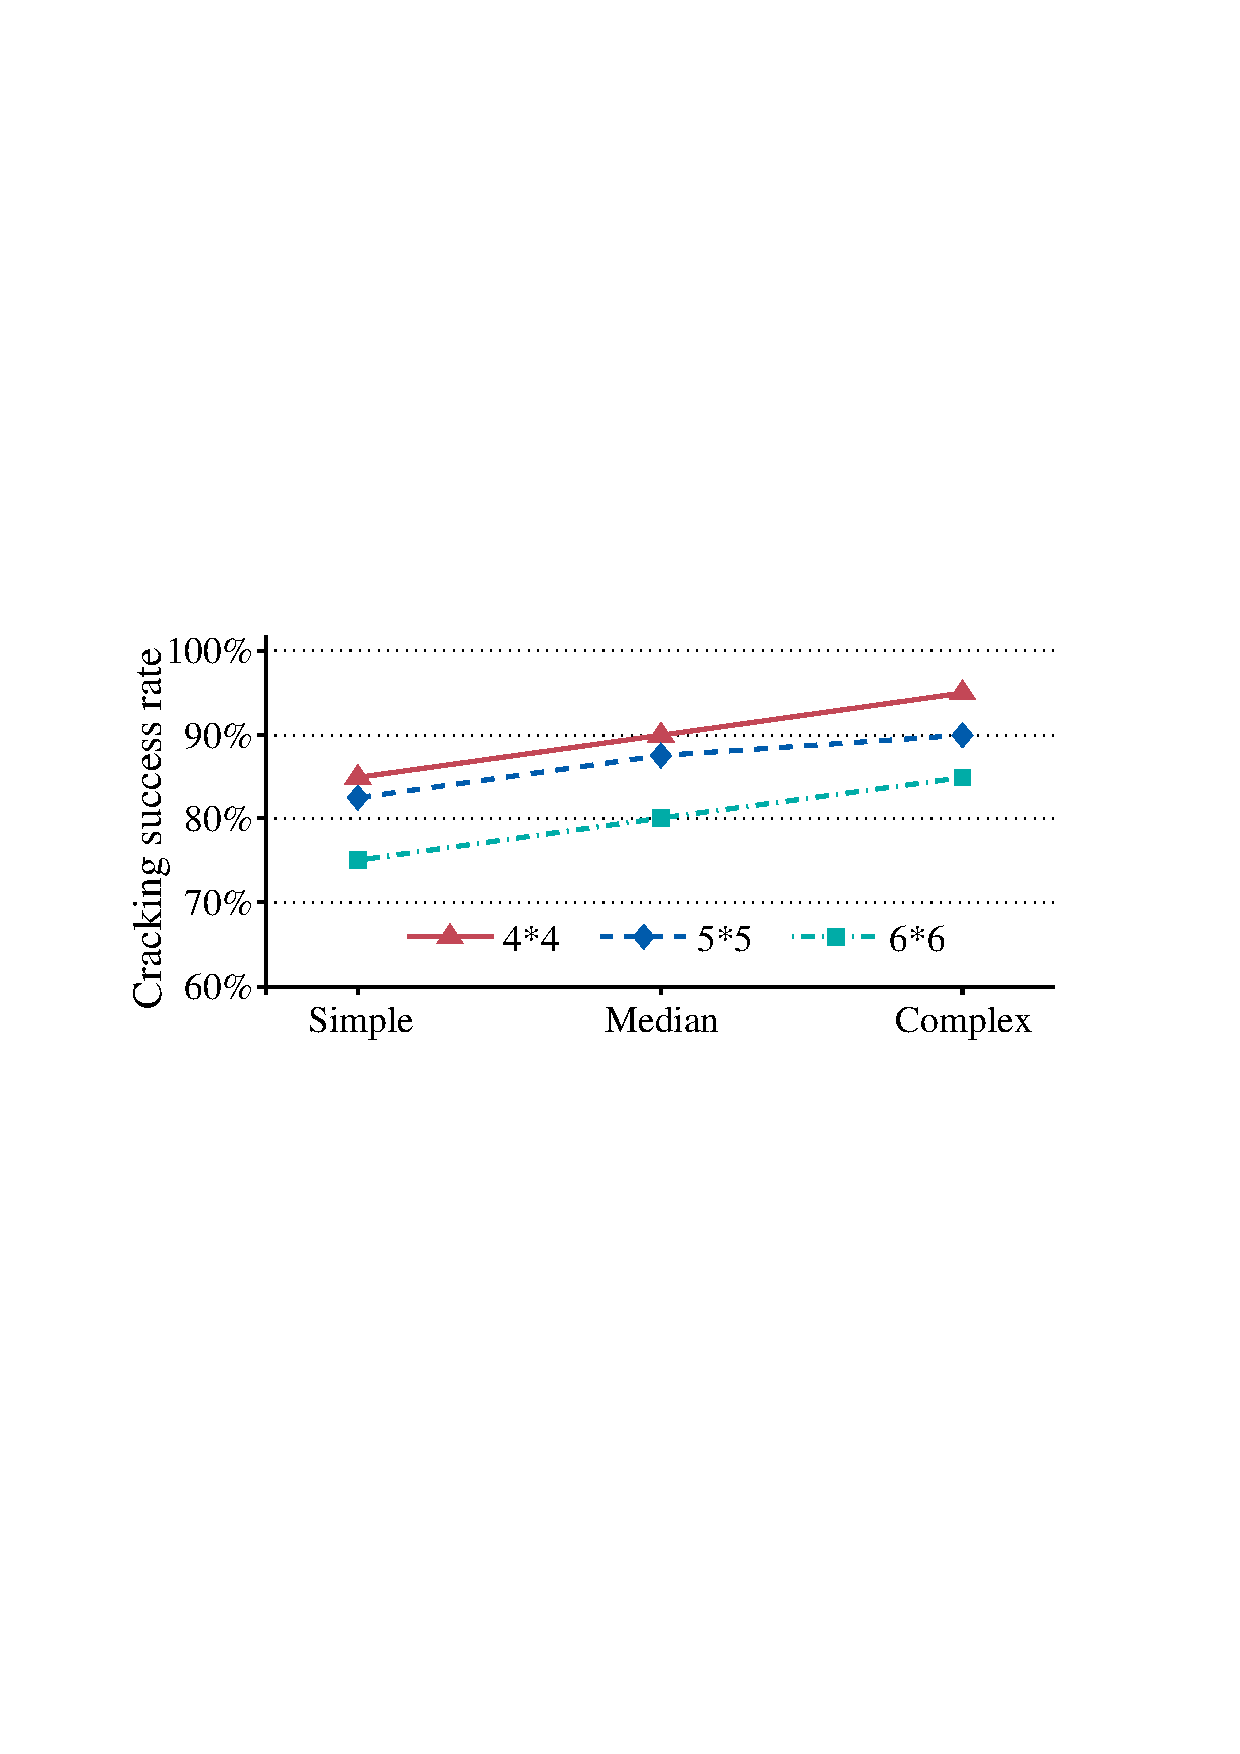
\includegraphics[width=0.35\textwidth]{fig/scalability.pdf}
            \vspace{-3mm}
            \caption{Success rates of our attack for different locking grids.}
            \vspace{-2mm}
            \label{fig:scalability}
            \vspace{-2mm}
        \end{figure}

    \subsection{Evaluation on Other Pattern Grids\label{sec:scalability}}
    \noindent \textbf{Result 8:} \emph{A pattern grid with more dots provides stronger protection but our attack can still crack most of the patterns.}

        There are a few applications (such as CyanLock) and customized ROMs available to increase the size of the pattern grid from $3\times3$ to $4\times4$, $5\times5$, and $6\times6$.
        Although a $3 \times 3$ grid remains
        a popular choice (as it is supported by the native Android OS), it is worth studying whether
        having more touch dots on a pattern grid leads to stronger security. In this
        experiment, we first ranked all possible patterns for each grid setting in
        ascending order according to their complexity scores. We then equally
        divided the patterns into three groups, simple, medium and complex,
        and asked our participants to randomly select 20 patterns from each group for evaluation. We
        report the success rate of our attack within five attempts. In the experiments, we have adapted our algorithms for each grid setting
        by adjusting the algorithm parameters (such as the line direction numbers).


        Figure~\ref{fig:scalability} shows the success rate of our attack
        for different grids. Similar to a $3 \times 3$ grid, our
        approach achieves a higher success rate for complex patterns over
        simple ones. On average, we can crack 90\% of the complex patterns.
        We observed that a grid with more dots does provide
        stronger protection. For complex patterns, the success rate of our
        attack drops from 95\% on a $4 \times 4$ grid to 87\% on a $6 \times
        6$ grid. For simple patterns, the success rate of our attack drops
        from 85\% on a $4 \times 4$ grid to 75\% on a $6 \times 6$ grid. This
        is because a fingertip trajectory can be mapped to a larger number of
        candidates on a grid with more dots. For instance, the pattern shown
        in Figure~\ref{fig:fig2} (f) can be mapped to 55
        candidate patterns on a $6 \times 6$ grid as opposite to 5 on a $3
        \times 3$ grid. Overall, our attack can crack over 75\% (up to 95\%)
        of the patterns within five attempts. One of the purposes of introducing
        pattern grids with more dots is to allow users to use more complex
        patterns. However, this experiment suggests that complex patterns remain less security on these grids under our attack.

        \begin{figure}[!t]
            \centering
            \subfigure{
                \begin{minipage}[t]{0.18\textwidth}
                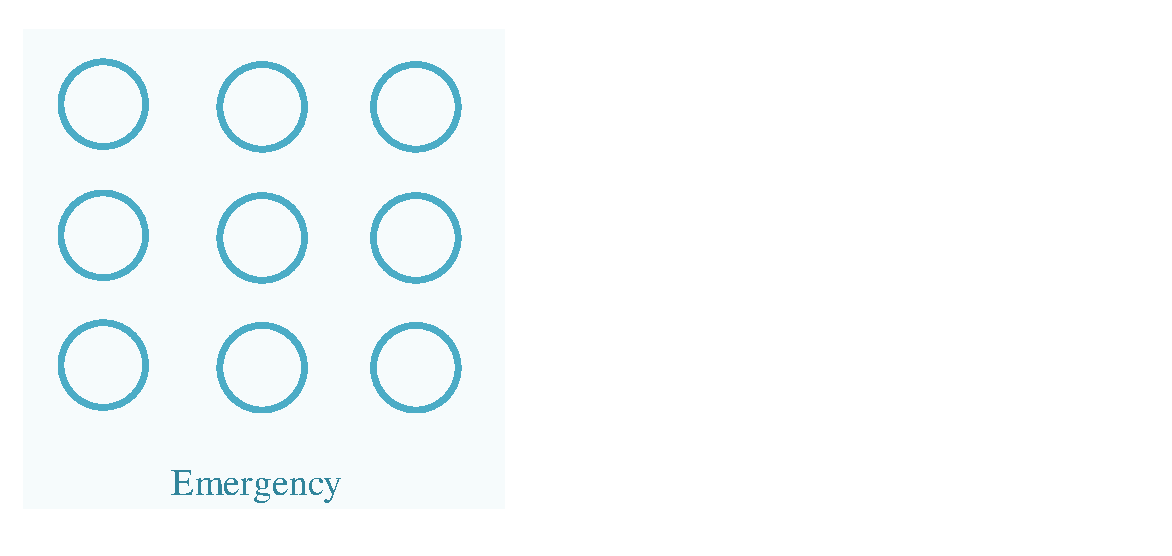
\includegraphics[width=\textwidth]{fig/pattern_screen.pdf}\\
                \centering \footnotesize (a) pattern-based interface
                \end{minipage}
            }
            \hspace{0.5cm}
            \subfigure{
                \begin{minipage}[t]{0.18\textwidth}
                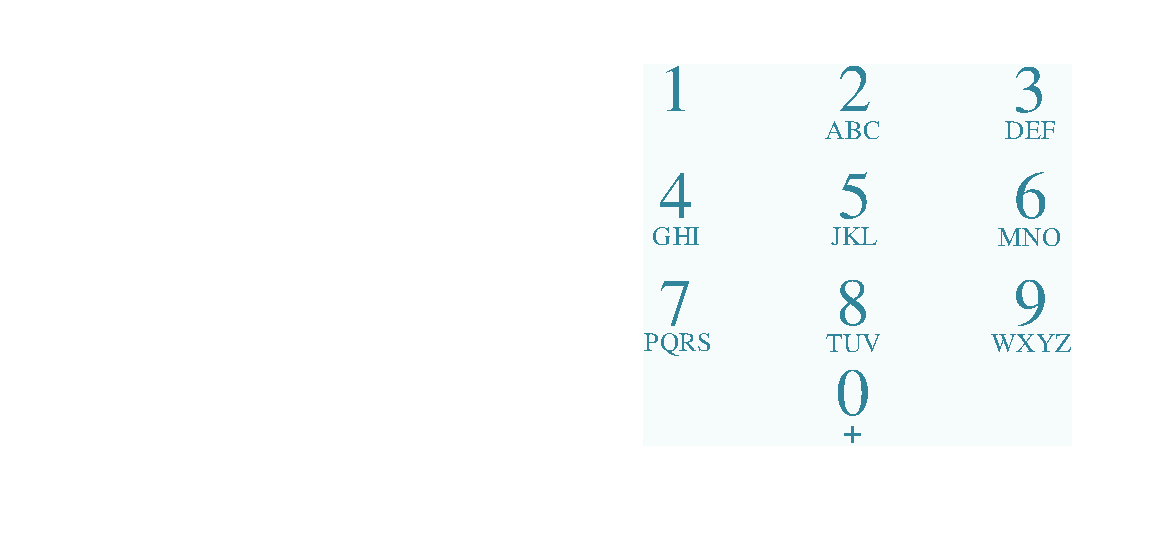
\includegraphics[width=\textwidth]{fig/pin_screen.pdf}\\
                \centering \footnotesize (b) pin-based interface
                \end{minipage}
            }
            \caption{Pattern-based and pin-based authentication interfaces from Xiaomi MI4 phone.}
            \label{fig:unlock interface}
        \end{figure}

    \subsection{\FIXED{Evaluation of Cracking PIN-based Passwords}}
        \noindent \textbf{Result 9:} \emph{PIN-based passwords are still vulnerable under our attack. This can be proved that we can break over 85\% of the passwords within five attempts using a simple variant method based on our approach.}

        Recall the basic idea of our attack, pattern lock can be reconstructed by tracking the fingertip movement  from the target video. Intuitively, out method can also infer to the PIN-base passwords by analyzing the pattern which is generated during unlocking the device. To prove this intuitively imagine, we total collected 30 4-digital PIN-based passwords. For each passwords, we ask our participants to keystroke the passwords on a Xiaomi MI4 phone. Figure~\ref{fig:unlock interface} shows the pattern-based and pin-based authentication interface of MI4 phone.  We use an IPhone4S phone to record the video respectively on the left-front, front and right-front of the target device from a distance of 2 meters.

        \noindent \textbf{Variant Methodology} There exists some differences between PIN-based passwords and pattern lock. These are summarized as follow: (1) PIN-base authentication interface has ten dots that is different from pattern lock, making the layout of interface of the two mechanisms different; (2) the dots on PIN-based interface can be typed repeated while they can only be visited once on pattern-base interface. The above two differentias make the structure of the pattern generated from PIN-based interface more complicated than the one from pattern-based interface. Our preliminary experiments suggest that we can reconstruct the trajectory of PIN-based password by connecting the touching points\footnote{Touching points are those points that tracked when fingertip touches the screen.}. We can get the location of touching point by the up-and-down motion direction of the fingertip inspired by the solution in~\cite{shukla2014beware}. To reconstruct PIN-based passwords, we increased the geometric information including both direction and length information to adjust the variant attack method. Figure~\ref{fig:pins_trajectory} shows the reconstructed fingertip trajectory using the variant method.

        \noindent \textbf{Results} Figure~\ref{fig:pin_results} shows the performance on cracking 4 digital passwords within different number of attempts. With first attempt, the success rate is only 53.3\% as most of tested passwords have two or more candidate patterns. As the increase of trial number, the success rate is significantly increased, and they respectively are 76.7\%, 80\%, 83.3\%, 86.7\% within 2, 3, 4, 5 attempts. Within five attempts, our method failed to crack four passwords. The reason that we failed two passwords is because they have more than five candidate patterns and for remaining two ones is that we detected the wrong location of one touching point due to the blue motion of the video footage. We believe that the expert attacker is able to improve the success rate using more attempts.



